\chapter{Methodology}

\section{Introduction to the framework} 
The following structure, which comprises a series of operations to be done on the data, is what we offer as a solution to these problems in order to solve them. Figure \ref{framework} is an illustration of the entire structure. The data collector and the inference engine are the two basic components that make up the framework. In the paragraphs that follow, I will dissect each part of the structure into its component phases. To make it simpler to keep track of where we are in the framework, we have allotted numbers to the several important stages (as indicated in the graphic below), and from this point on, we will refer to these labels instead of the descriptions.

Our whole pipeline includes all of the essential components and systems to comprehensively handle the problem. As a result of the modular design of the framework, it is feasible to replace any one of the individual stages with a different implementation if this proves to be necessary. Because of its scalability, the system may be applied to the management of extremely large datasets. The structure is designed to function regularly even if some processing steps experience errors. This is made possible by the framework's construction. A distributed design was used in the development of the framework so that it may be utilised on a broad range of computer systems. The framework's ability to readily include more procedures as they become necessary is made possible by the modular nature it possesses.

\newpage
\begin{landscape}
\begin{figure}[t]
  \noindent 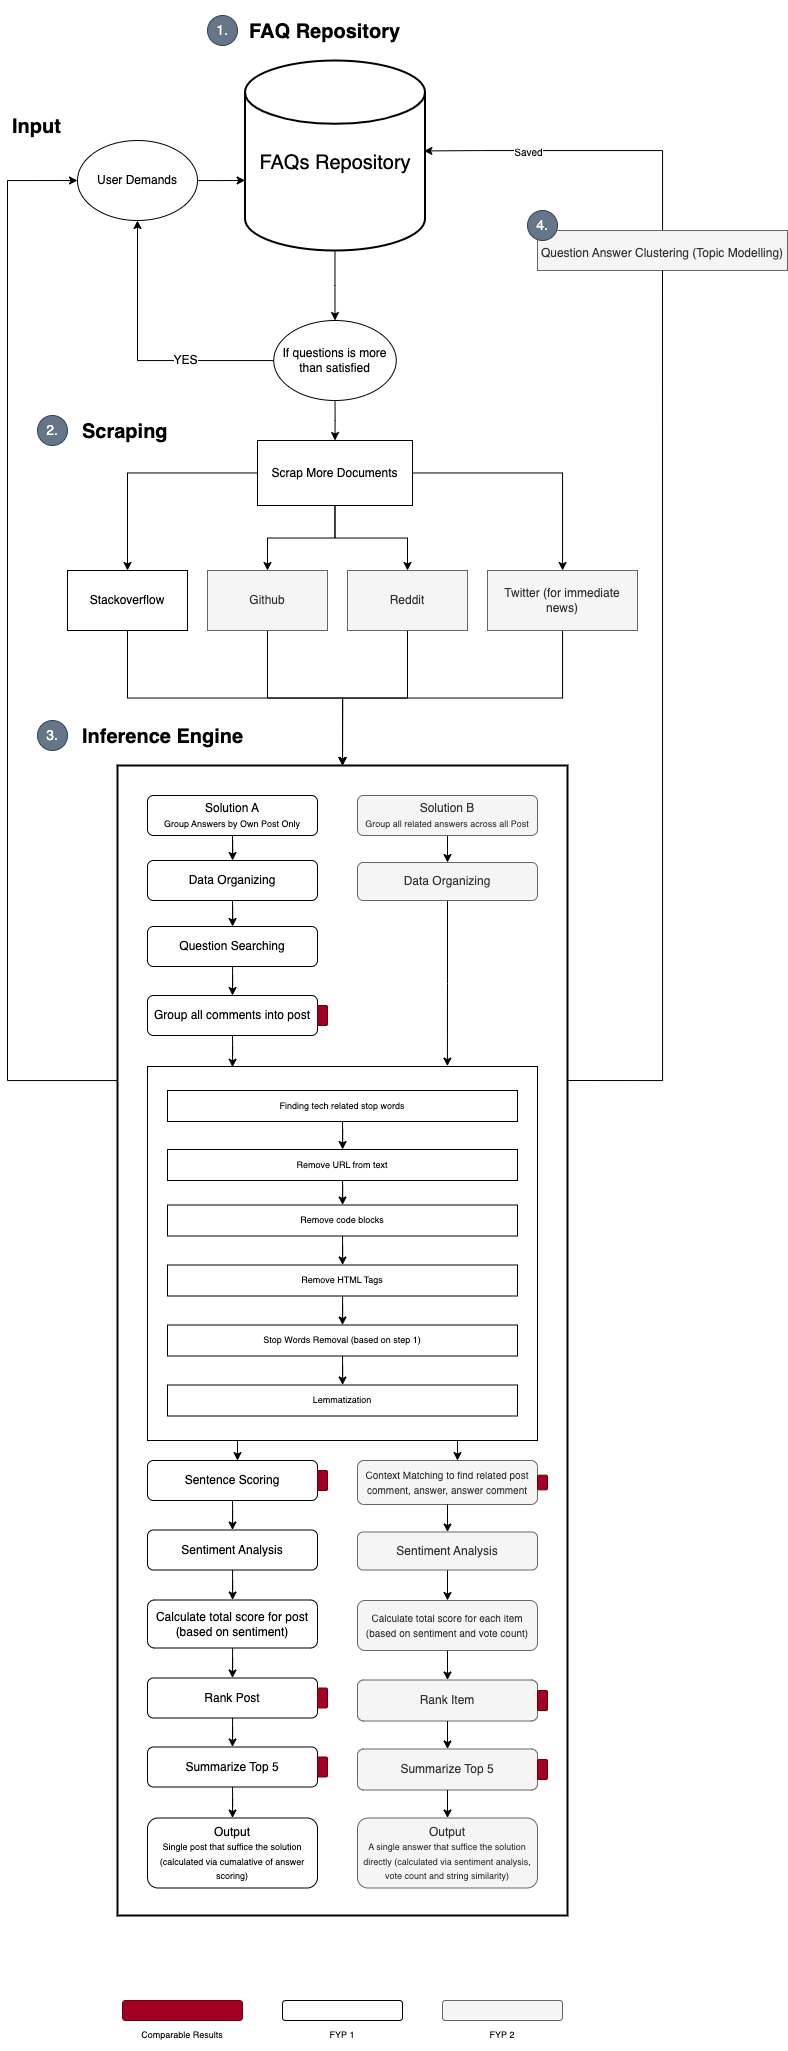
\includegraphics[scale=0.28, angle=0]{Framework.png}
\caption{Framework}\label{framework}
\end{figure}
\end{landscape}
\newpage

\section{Introduction}
In the following, we will go through everything that led us to the suggested framework. This will include a discussion of the ways in which the data are prepared, studied, and processed, as well as an evaluation of the approach that was developed as a consequence.

\section{Data Collection (Scraping) -- 1.0}
To begin presenting the framework, we must first have access to the dataset; without it, we will be unable to provide proofs or draw conclusions about the suggested framework. For us, the dataset is vital since it determines the good or bad of the assessment process. 

According to our suggested framework \ref*{framework}, we have four primary data sources for datapoints: Stack Overflow, GitHub (Issues), Reddit, and Twitter. Four of these provide us with data that is fairly distinct. The data on Stackoverflow is in the form of questions and answers, but the data on GitHub is in the form of code majority speaking. Reddit data is more likely to contain chained responses, whereas Twitter data is more likely to have rapid, real-time updates.

In terms of FYP1, Stackoverflow will be our primary data source because it makes it much easier for us to demonstrate whether or not our method works. As a result, we'll be collecting our information from Stack Overflow.

We utilised the stack overflow api to locate relevant topics on stackexchange depending on the developer's query. We generate an API token on the Stack Overflow gateway since the API is not publicly available.

The Stack Exchange API is a RESTful API that allows you to access data from Stack Exchange sites. It is a read-only API, which means that you can only retrieve data from the sites, not modify it. The API is available at api.stackexchange.com/docs. You can use the API to retrieve data from Stack Exchange sites in a variety of formats, including JSON, XML, and JSONP. We'll be quering the data in JSON format. 

\pagebreak
Example of a query to the Stack Exchange API:
\begin{lstlisting}
  {
    "tags": [
    "node.js",
    "reactjs",
    "react-hooks"
    ],
    "owner": {
    "account_id": 26363344,
    "reputation": 9,
    "user_id": 20019220,
    "user_type": "registered",
    "profile_image": "https://lh3.googleusercontent.com/...",
    "display_name": "George Prethesh",
    "link": "https://stackoverflow.com/users/20019220/george-prethesh"
    },
    "is_answered": false,
    "view_count": 27,
    "answer_count": 3,
    "score": 0,
    "last_activity_date": 1674042867,
    "creation_date": 1674039763,
    "question_id": 75158231,
    "content_license": "CC BY-SA 4.0",
    "link": "https://stackoverflow.com/questions/75158231/..",
    "title": "React useEffect OnSubmit Rendering Post api multiple times"
    },
\end{lstlisting}

The accompanying screenshot displays the response from the Stack Exchange API call. As you can see, it provides us with a number of useful pieces of data, including the tags, owner, title, link, and many more besides, however in this instance we are just concerned with the tags and the link. We may use the link to open a new browser tab and copy and paste the information from the website.

To do so automatically without human inteference, we will need to resort to the scraping technique in order to get the necessary information from the relevant web sites. Because of this, selenium is essential.

Selenium is a free (open source) automated testing suite for web applications across different browsers and platforms. It is used to automate web applications for testing purposes, but is certainly not limited to just that. Bots that perform web scraping, data mining, load testing, network traffic recording, and screen scraping are all common uses for the tool. Selenium is a portable framework for testing and automating web applications. Selenium provides a playback tool for authoring tests without learning a test scripting language (Selenese). It also provides a test domain-specific language (Selenium-IDE) to write tests without learning a general-purpose programming language. The tests can then run against most modern web browsers. Selenium runs on Windows, Linux, and Mac OS X. Selenium is open source software released under the Apache 2.0 license.

However, there is a problem since most websites nowadays use anti-bot procedures to block automated programmes. Since our scraper may be blocked from accessing a Cloudflare-protected website, this complicates web scraping.

Therefore, we need to combine selenium with the ultrafunkamsterdam created and maintained python package undetected chromedriver to properly exploit its potential. This bundle is a selenium wrapper that enables us to utilise selenium without being noticed by the website. The website will deny us access if it discovers that we are using selenium, so knowing this is crucial.

When all of that is complete and in place, we can proceed to scrape all of the posts. The python code is designed to be error fail save, with the bulk of the code wrapped inside try catches blocks, so that if an error does occur, it will not stop the current process. This is critical since we'll be extracting more than 200-300 posts most of the time.

The list of our items of interest is as follows:
\begin{itemize}
    \item Post id
    \item Post link
    \item Post Title
    \item Post Body
    \item Post date
    \item Post Votecounts
    \item Comment id
    \item Comment score
    \item Comment username
    \item Comment text
    \item Comment Date Time
    \item Answer id
    \item Answer Text
    \item Answer Body
    \item Answer Date Time
    \item Answer Votecounts
    \item Answer Comment id
    \item Answer Comment Text
    \item Answer Comment Body
    \item Answer Comment Date time
    \item Answer Comment Votecounts
\end{itemize}

Because Selenium has a capability called "Find Element," it is quite easy for us to zero in on all of the components that are of interest. The information is structured in a manner similar to that of a dictionary, with the post id acting as the key and a list of all objects of interest performing the function of the value. After that, the data with the modifications are saved as a csv file. It is important to take note that the CSV file has a separate row for each comment, response, and response comment. This is due to the fact that we want to do a more in-depth review of the data.

We are going to scrape articles that include the word "React UseEffect" in order to acquire the necessary data. As a direct result of this, we now have a.csv file that has 3336 rows and 22 columns.

Notably, the web scraper is programmed to run once per day in order to provide us with the most recent data possible. This is necessary since data is always shifting, and we aim to compile the most up-to-date information possible. In addition to this, the scraper will be housed on a server so that it may expand as the needs of the business dictate.


\section{Data Cleaning} \label{data-cleaning}
It is important to note that the data is not perfect. There are some null values that need to be addressed. The following are the null values that need to be addressed:

\noindent  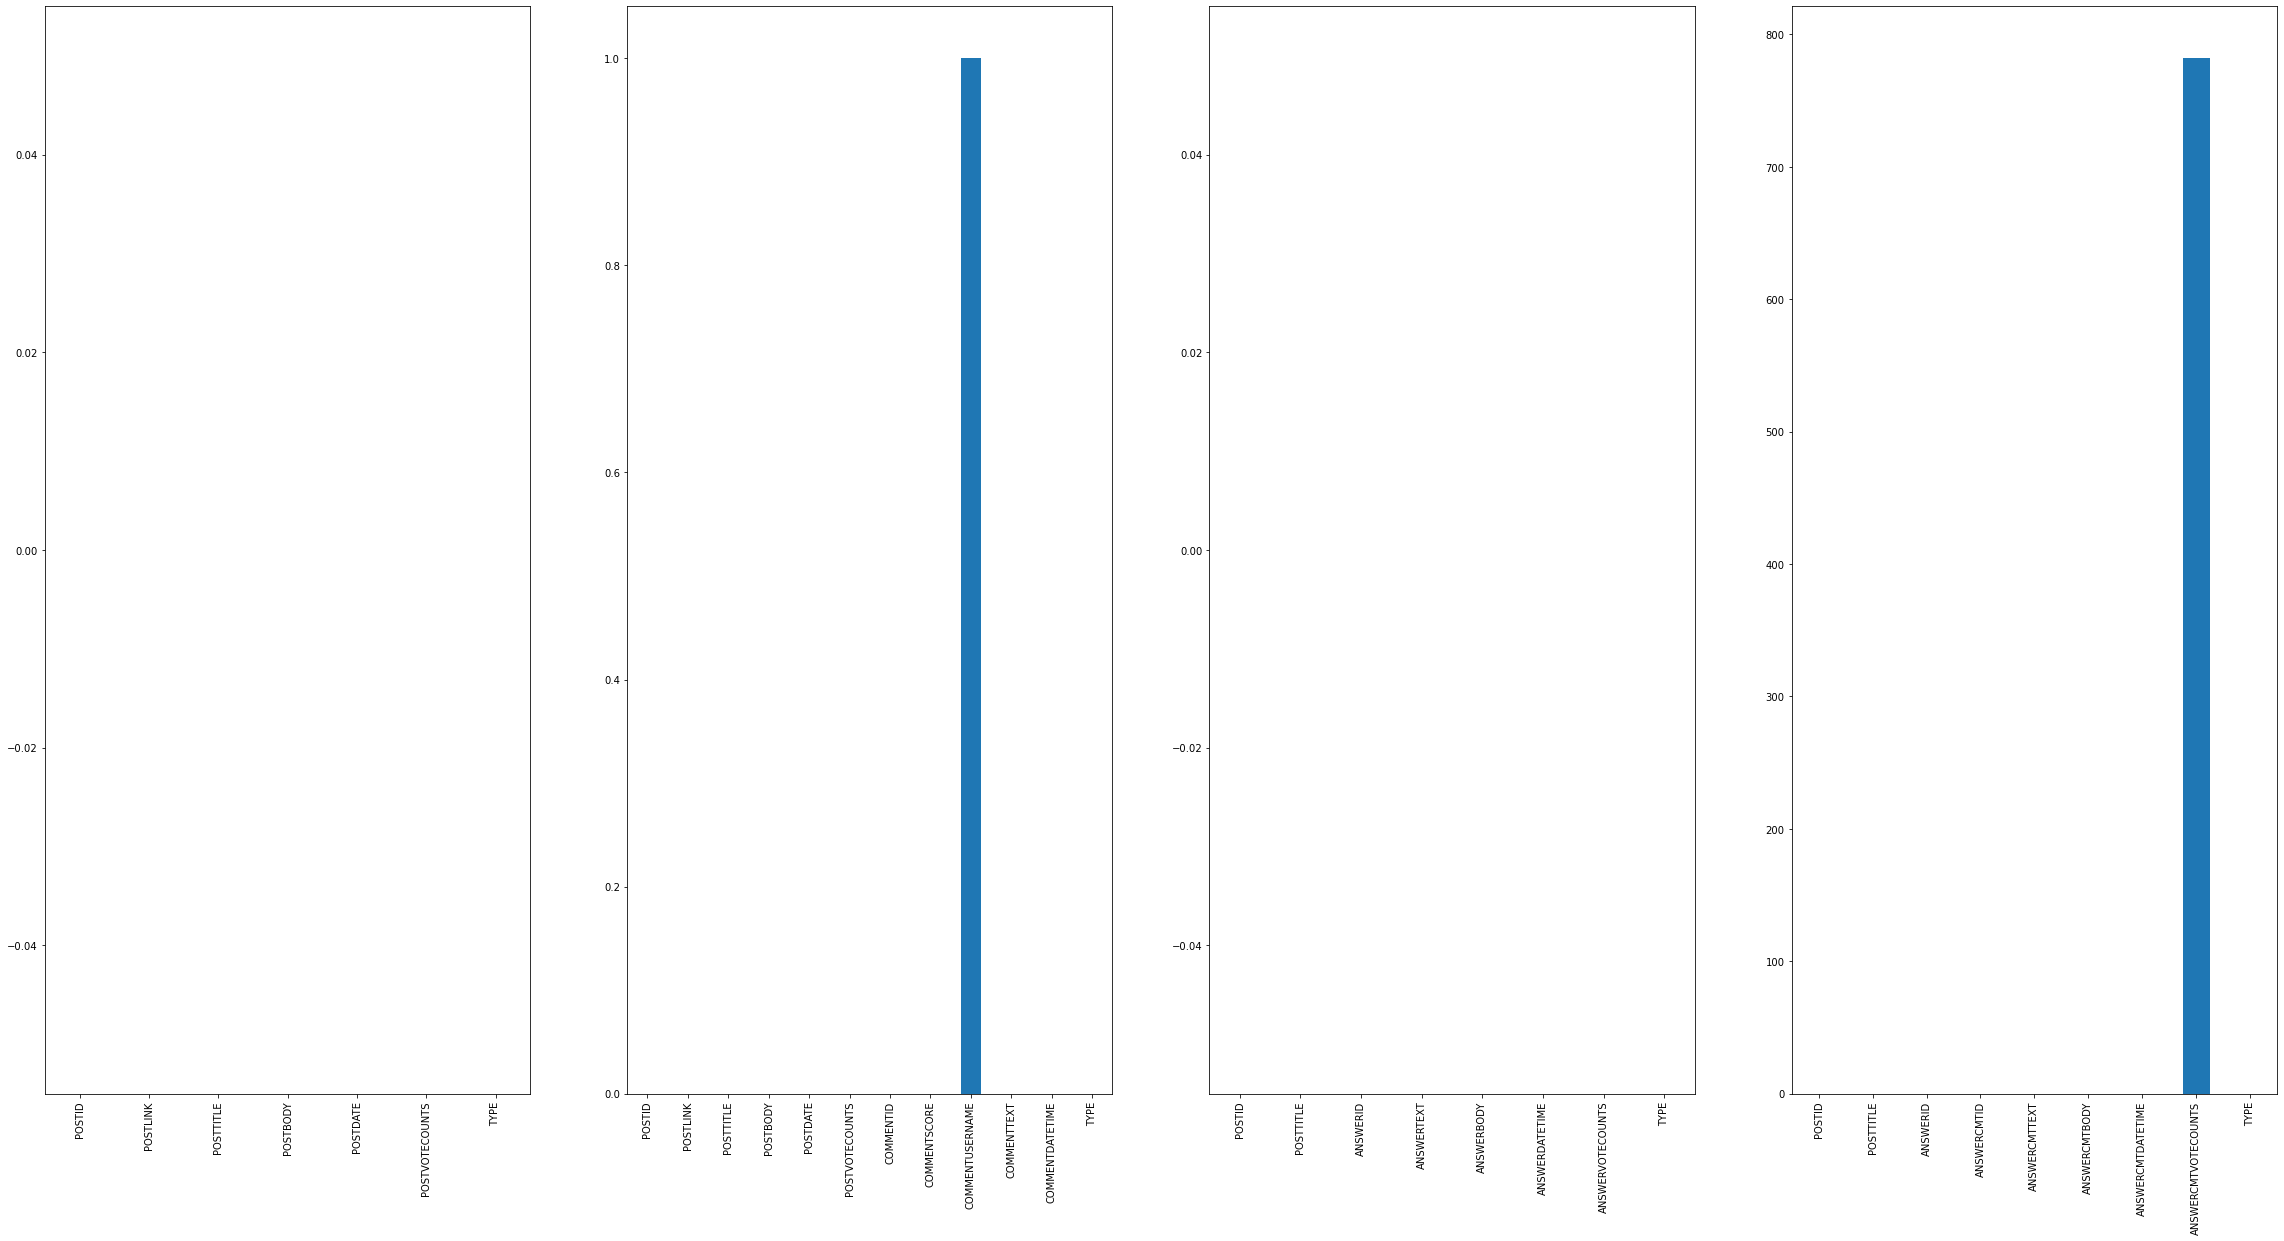
\includegraphics[scale=0.25, angle=90]{null-values-1.png}\\

From the diagram we can see that everything is perfect except two columns namely the Comment\_Score and Answer\_Comment\_Score. The reason for this is that the comments and answer comments do not have a score. With that being said, we can replace the null values with 0. The following is the result of the replacement:
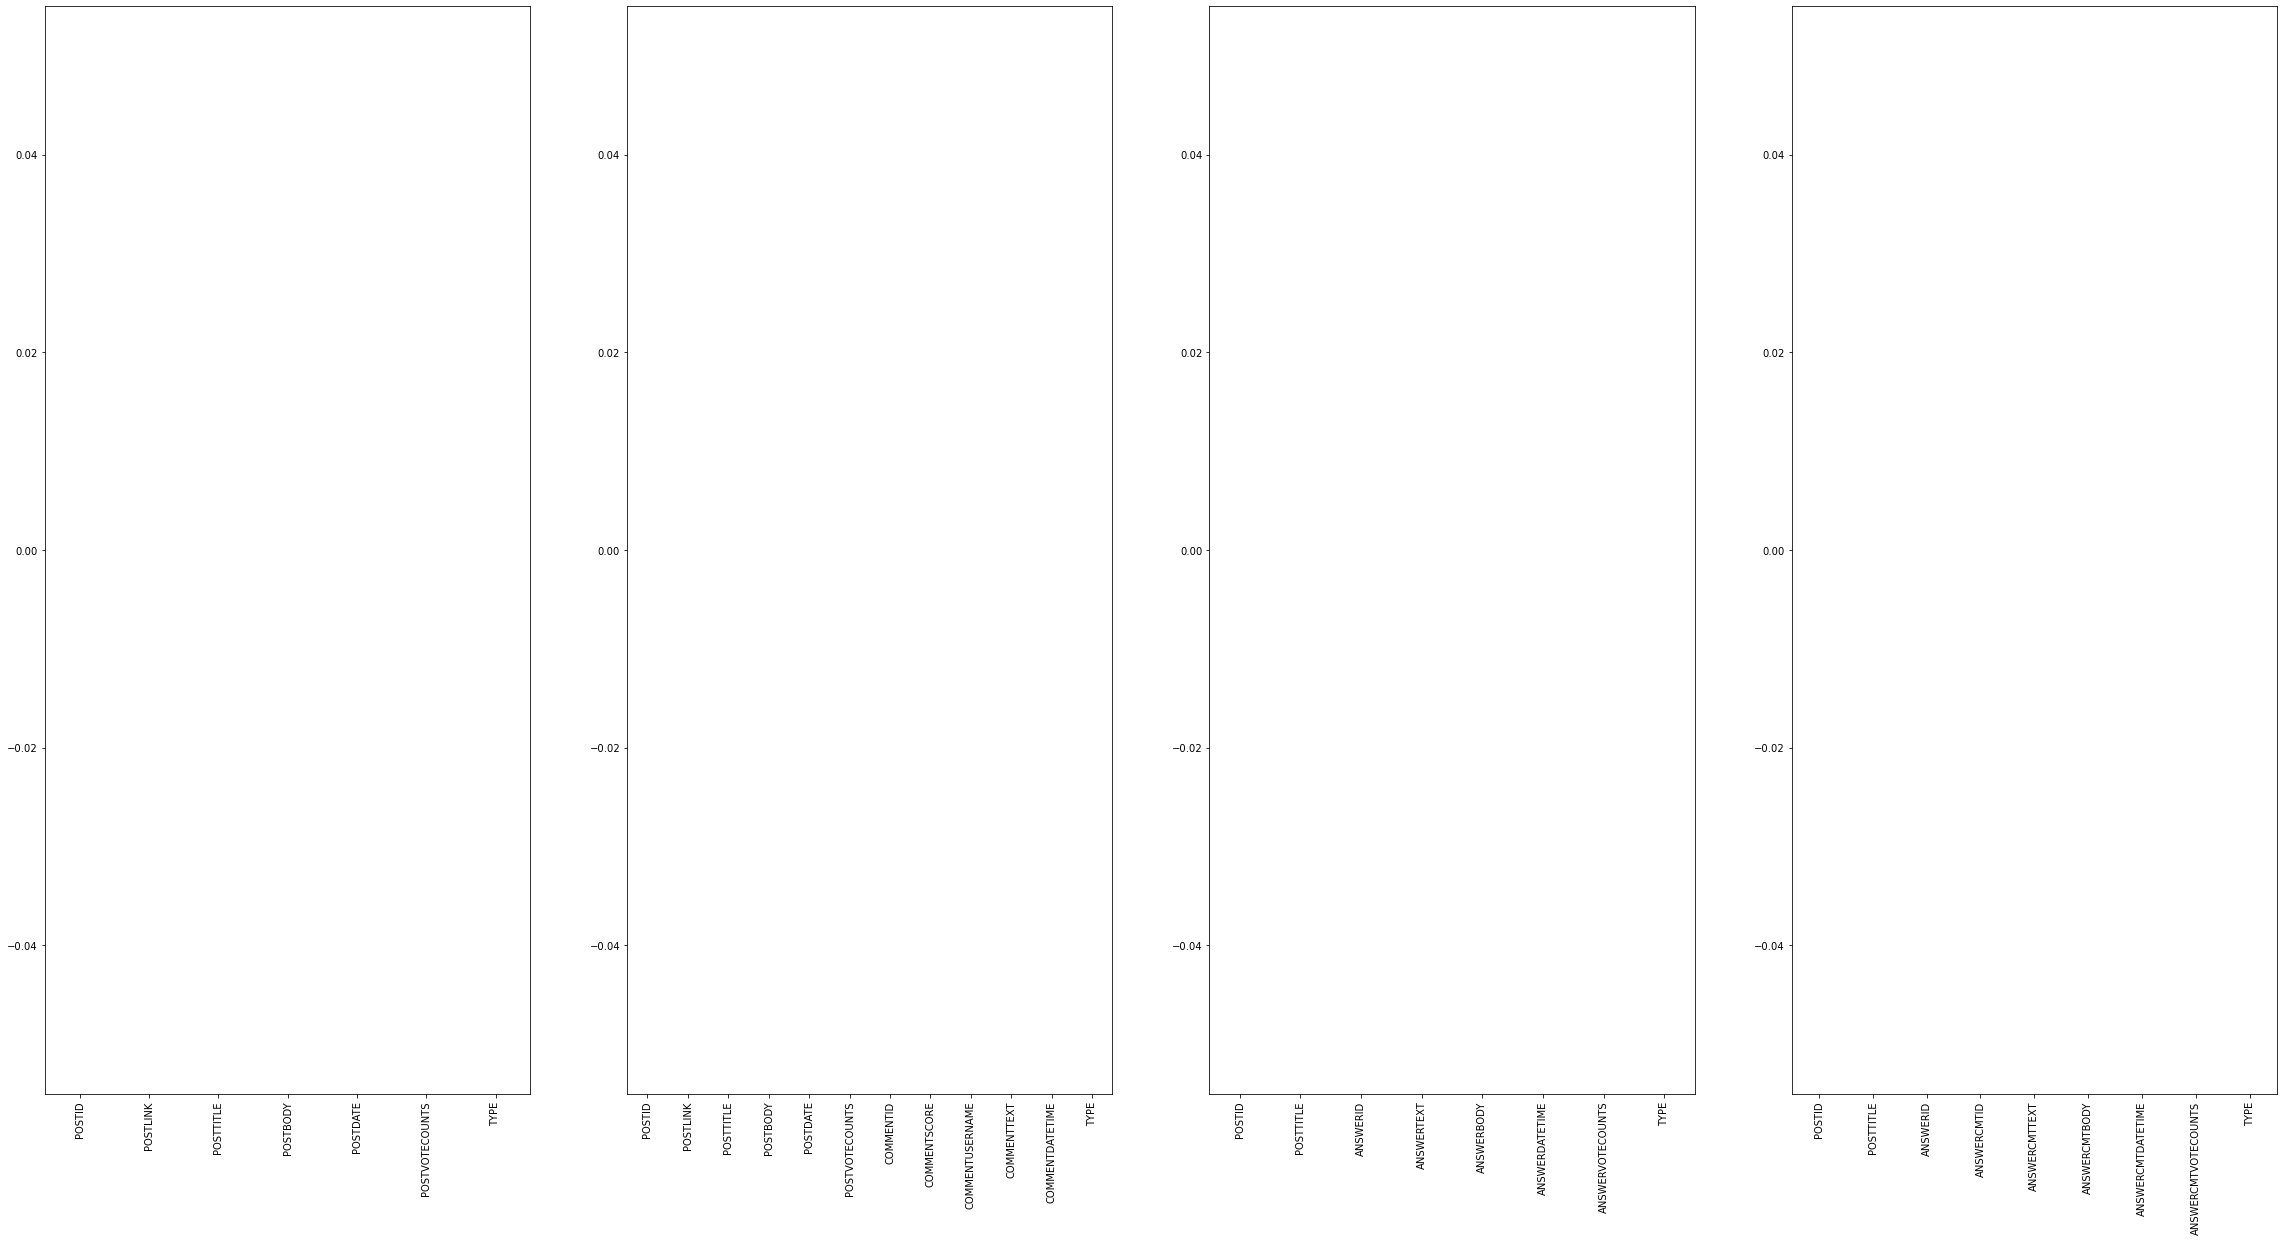
\includegraphics[scale=0.25, angle=90]{null-values-2.png}\\

\section{Data Exploration}
It is usually a good idea to examine the data rather than just skim at it, so always do both.

First we should look at how many unique title there are. This is important since we want to make sure that we have enough data to work with. After analyzing the data, we can see that there are 660 unique titles. This is a good sign since it means that we have enough data to work with.

In order to analyze the longetivity of the current topic on stackoverflow, we will plot the time span distribution of all postings as a whole.

\noindent  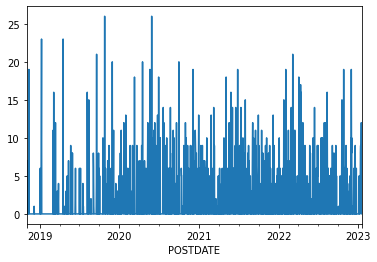
\includegraphics[scale=1]{post-time-distri.png}\\

As you can see, the number of posts per day is pretty constant. This is a good sign since it means that the number of people using the React UseEffect is still there and therefore it might gives us a better result.

Next, we will look at the votecounts distribution across all of the dataset as a whole, it is important to note that the votecounts is the number of votes that a post has received, the higher the votecounts, the more popular the post is. We can probably inference that the more popular the post is, the more likely it is to be answered, and the more likely it is to be answered, the more likely it is to be answered correctly.

\noindent 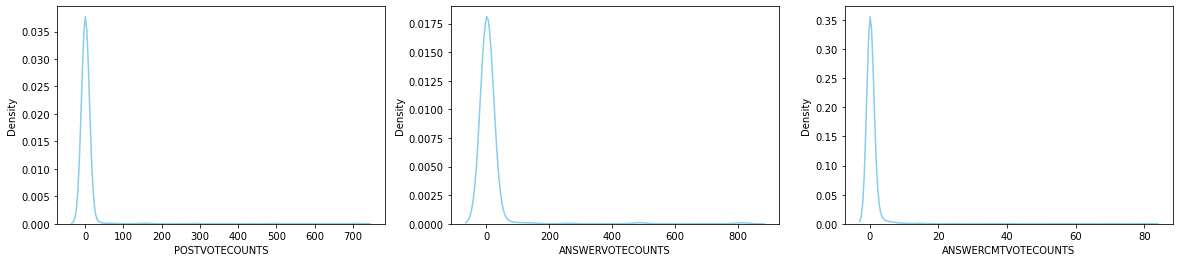
\includegraphics[scale=0.35]{votecounts-distri.png}\\

As you can see, the distribution is skewed to the left. This is not a good sign as it means that the majority of the posts have a low votecounts. With that being said, this motivates us to explore more data to be mined from the dataset and facilitate to our work.

\section{Inferencing Engine -- 2.0}
We've attempt to propose an inference engine which will handle the core parts of the system. Everything from preprocessing, sentence scoring, and sentence selection will be handled by the inference engine. With the below diagram, it is a close up view of the inference engine. We'll be going through each of the components and explain what they do.

\noindent 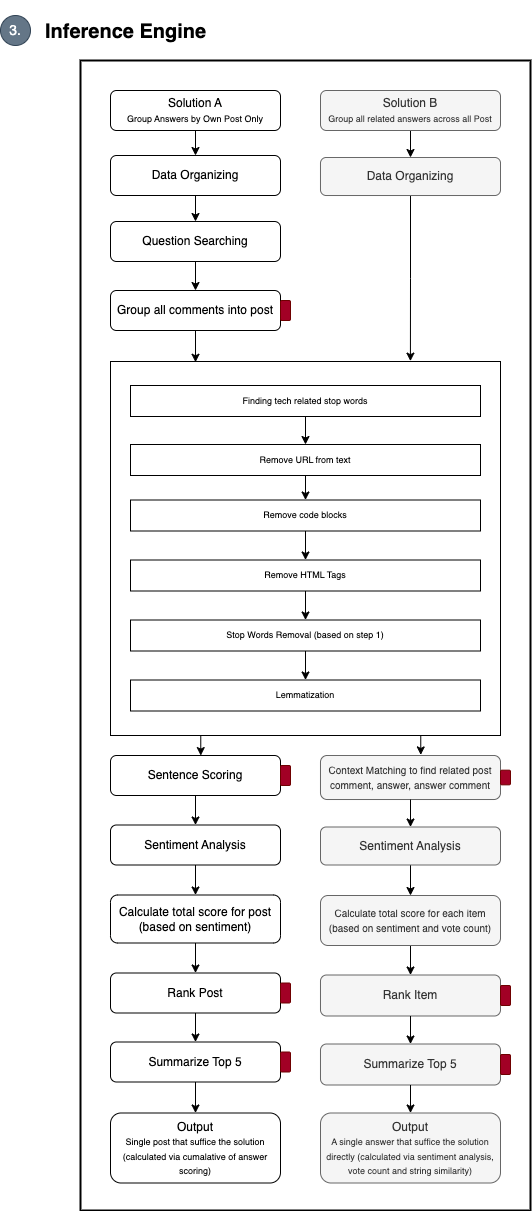
\includegraphics[scale=0.6]{inference-eng.png}\\

In the proposed inference engine system, we came up with 2 ideas to solve the problem, the one highlighted in green in color is solution A meanwhile the one highlighted in purple is solution B. In FYP 1, we'll be only implementing solution A, but we'll be explaining both of them in detail and the pros and cons of each of them.

\subsection{Solution A}
Posts titles are usually short and concise, and they are usually the first thing that people see when they are looking for a solution to their problem. Therefore, it is intuitive to assume that the title of the post tells us what the post is about. With that being said, this proves that all comments and answers should be incapsulate in the post itself, and the post should be view as a whole when we perform ranking. This is the idea behind solution A. Essentially, we're ranking the posts incorporating the comments and answers into the post itself.

\subsection{Solution A - Architecture}
A close up view of the architecture of solution A can be seen in the following figure~\ref*{solution_a_architecture}.

\pagebreak
\begin{figure}[H]
  \centering
  \noindent 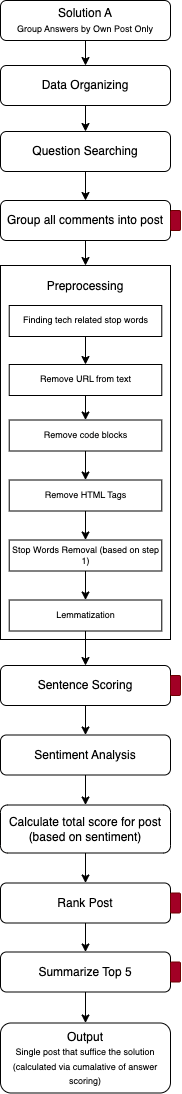
\includegraphics[scale=0.75]{assets/solution-a.png}
\caption{Solution A Architecture }\label{solution_a_architecture}
\end{figure}

\subsubsection{Data Organizing} \label{data-organization}
First, we need to sort the information into the appropriate buckets. Posts, comments, answers and answers comments are the four primary types of information we separate apart. The goal here is to facilitate our work with the data. The reason for this is that the data in the csv is not organized in a way that is conducive to our work, we can see that in the following diagram:

\noindent So essentially we went from this: 

\noindent 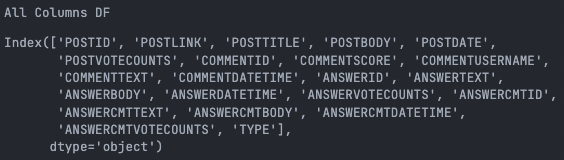
\includegraphics[scale=0.65]{all_columns_df.png}\\

\noindent To this:

\noindent 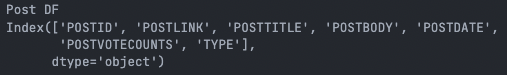
\includegraphics[scale=0.65]{post_df.png}\\
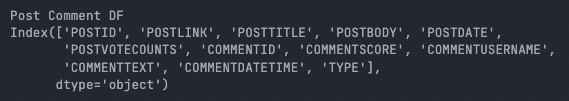
\includegraphics[scale=0.65]{post_comments_df.png}\\
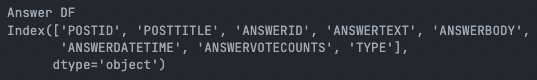
\includegraphics[scale=0.65]{answer_df.png}\\
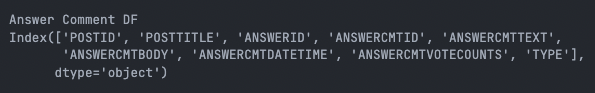
\includegraphics[scale=0.65]{answer_comment_df.png}\\

\subsubsection{Matching Posts based on String Similarity}
The first step is to match the posts based on string similarity. This is done by using the python package fuzzywuzzy. Fuzzy Wuzzy is a Python library for doing approximate and partial string matching using Levenshtein distance. 

There are two methods we've used in fuzzy wuzzy, the first one is the partial ratio method, which is used to compare the similarity of two strings. fuzz.partial\_ratio(str1, str2) method compares two strings and returns a score between 0 and 100, indicating the similarity of the two strings. The score is based on the longest contiguous matching substring between the two input strings.

fuzz.token\_sort\_ratio(str1, str2) method also compares two strings and returns a score between 0 and 100, indicating the similarity of the two strings. The score is based on the number of matching tokens (i.e., words) between the two input strings, after sorting the tokens alphabetically in both input strings.

In short, partial\_ratio checks for longest matching substrings and token\_sort\_ratio checks for matching tokens after sorting them alphabetically.

The reason for this is to better match the posts with the developer requirements. But we did not stop there, Fuzzy Wuzzy is entirely based on levenshtein distance, which is a metric for measuring the difference between two sequences. The levenshtein distance between two words is the minimum number of single-character edits (i.e. insertions, deletions or substitutions) required to change one word into the other. This might introduce some issues as the levenshtein distance is not perfect. For example, the levenshtein distance between "react" and "reactjs" is 2, which is not ideal. 

Another string similarity method is then proposed, namely spaCy, which is a free, open-source library for advanced Natural Language Processing (NLP) in Python. It is designed specifically for production use and helps to build applications that process and “understand” large volumes of text. 

The notable differences between FuzzyWuzzy and spaCy are:
\begin{itemize}
    \item FuzzyWuzzy is based on Levenshtein distance, which is a metric for measuring the difference between two sequences. The levenshtein distance between two words is the minimum number of single-character edits (i.e. insertions, deletions or substitutions) required to change one word into the other.
    \item spaCy is based on word embeddings, which is a type of word representation that allows words with similar meaning to have a similar representation. Word embeddings are a type of word representation that allows words with similar meaning to have a similar representation. It is a distributed representation for the text that is perhaps one of the key breakthroughs for the impressive performance of deep learning methods on challenging natural language processing problems.
    \item  FuzzyWuzzy is faster than spaCy, but spaCy is more accurate.
    \item  FuzzyWuzzy is more suitable for matching short strings, while spaCy is more suitable for matching long strings.
\end{itemize}

To further filter out the results, we only take the results that have a score of 50 and above, as the results with a score below 50 are not relevant to the developer requirements, and we do not want to waste our time on them. 

To test the accuracy of the two methods, we've prompted a random query --  \textbf{"Useeffect hook rerenders infinitely" }, and we've compared the results of the two methods. Just for context there are 660 unique posts in the dataset.

The result is very contradictory, as the result of FuzzyWuzzy gives us a whopping 112 matches, while the result of spaCy gives us 58 matches. But if we take a closer look, we can see that the result of FuzzyWuzzy is more accurate, as the result of Spacy contains a lot of false positives, some of the matches are even unrelated to the developer requirements. 

\begin{figure}[H]
  \noindent 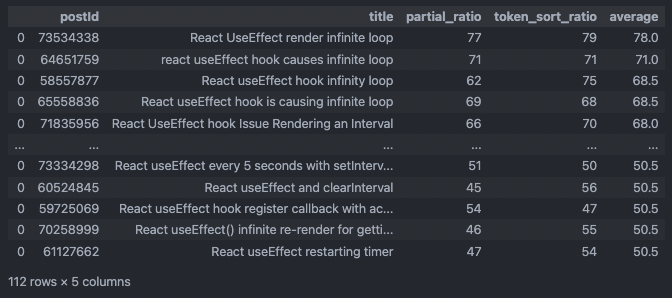
\includegraphics[scale=0.65]{assets/fuzzy-wuzzy-query-1-results.png}
\caption{Fuzzy Wuzzy Results on the query "Useeffect hook rerenders infinitely"}\label{fuzzy_wuzzy_query_1_results}
\end{figure}

\begin{figure}[H]
  \noindent 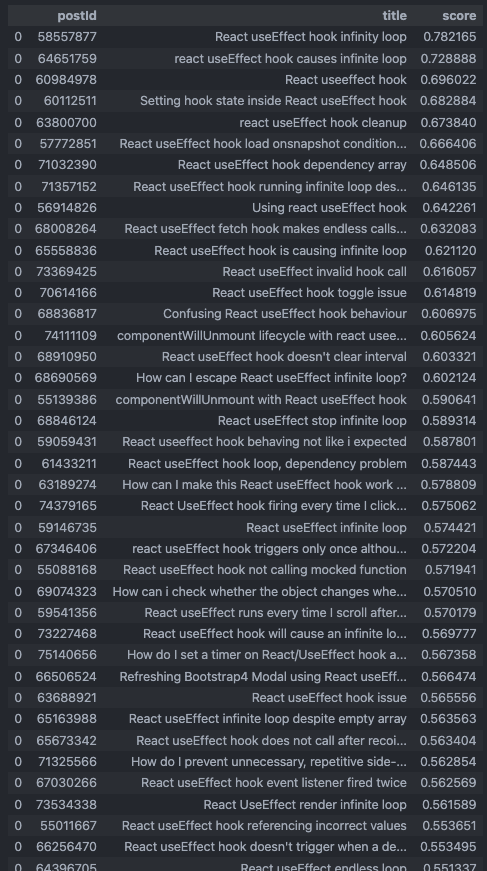
\includegraphics[scale=0.45]{assets/spacy-query-1-results.png}
  \noindent 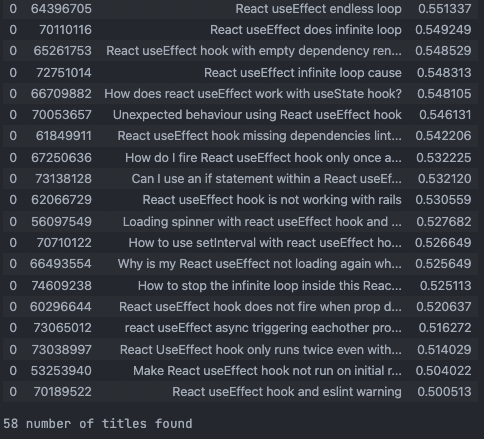
\includegraphics[scale=0.45]{assets/spacy-query-1-results-1.png}
\caption{Spacy Results on the query "Useeffect hook rerenders infinitely"}\label{spacy_query_1_results}
\end{figure}

However more testings needed to be taken place to truly crown the winner. Hence, we move forward to test the capabilities of both models using another query prompt, this time around we went for a longer sentence -- \textbf{"How to solve useEffect hook rerenders infinitely?" } 

This time around, the result is more or less on the same ratio, as the result of FuzzyWuzzy gives us 132 matches, while the result of spaCy gives us 195 matches.

\begin{figure}[H]
  \noindent 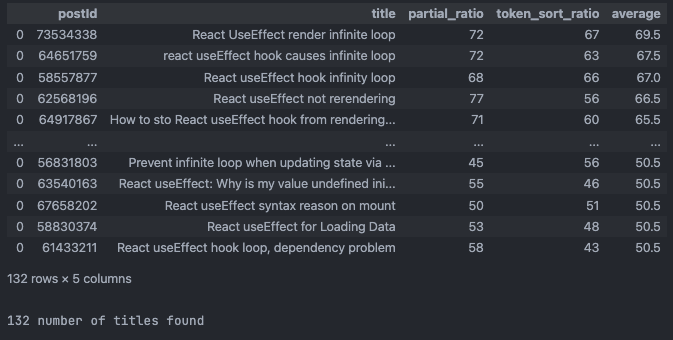
\includegraphics[scale=0.65]{assets/fuzzy-wuzzy-query-2-results.png}
\caption{Fuzzy Wuzzy Results on the query "How to solve useEffect hook rerenders infinitely?"}\label{fuzzy_wuzzy_query_2_results}
\end{figure}

\begin{figure}[H]
  \noindent 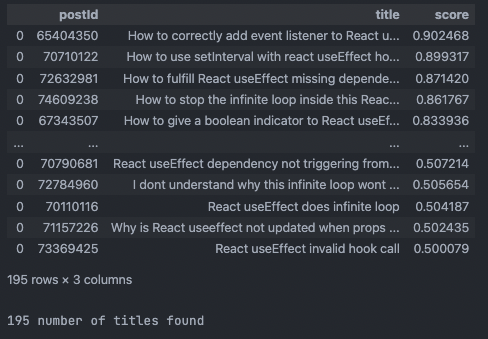
\includegraphics[scale=0.65]{assets/spacy-query-2-results.png}
\caption{Spacy Results on the query "How to solve useEffect hook rerenders infinitely?"}\label{spacy_query_2_results}
\end{figure}

At this point, it is clear that Spacy is more accurate than FuzzyWuzzy, but it is also clear that FuzzyWuzzy is faster than Spacy. Hence, we decided to use both methods to filter out the results, and we will use the results that are common between the two methods.

\subsubsection{Group all answers, comments, and answer comments by post\_id} \label{grouped_by_post}

The next step is to group all answers, comments, and answer comments by post\_id, so this way, all answers, comments, and answer comments can be concatinated into a single dict with the post\_id as the key, and thus all answers, comments, and answer comments can be viewed as a single string. Viewing everything as a single string is crucial for us as it's way easier to do sentence scording, sentiment analysis and other NLP tasks on a single string than on a list of strings. For that to happen we create a class called \textbf{GroupedComments} which is responsible for grouping all answers, comments, and answer comments by post\_id.

% write code blocks
\begin{lstlisting}[language=Python]
class GroupedComments: 
  def __init__(self, title, post, post_comments, answers, answer_comments): 
      self.title = title
      self.post = post
      self.post_comments = post_comments
      self.answers = answers
      self.answer_comments = answer_comments
\end{lstlisting}

We then use a simple python script that iterates over the data and groups all answers, comments, and answer comments by post\_id. The disctionary can be visualized as follows:

\pagebreak
\begin{lstlisting}[language=Python,caption={Grouped Comments Dictionary Example},captionpos=b]
  "post_id": {
    "title": "title",
    "post": "post",
    "post_comments": "post_comments",
    "answers": "answers",
    "answer_comments": "answer_comments"
  }
\end{lstlisting}

Since now that the data has been formatted nicely it is very easy for us to track the context of the data and to do further analysis on the data.

\subsubsection*{Rank Post - 1st Round}
With all of the comments grouped together we can begin our first analysis on the data. The context of the ranking this round is that, all of the comments, answers, answers comments are grouped under the individual parent posts, and the posts are ranked by the similarity score between the query and the post.

\begin{figure}[H]
  \noindent 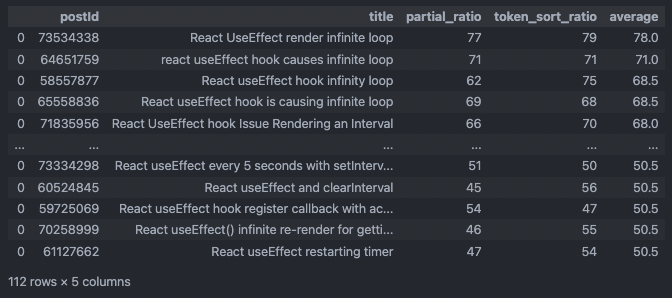
\includegraphics[scale=0.65]{assets/fuzzy-wuzzy-query-1-results.png}
\caption{Rank Post - 1st Round}\label{rank_post_1st_round}
\end{figure}

\subsubsection{Preprocessing - Finding tech related stop words} \ref{sssec:preprocessing_finding_tech_related_stop_words} \label{sssec:preprocessing_finding_tech_related_stop_words}
The next step is to find tech related stop words. This is done in order to remove the stop words from the data. Stop words are words that are not important to the data, and they are usually words that are used frequently in the data. 

However, finding stop words is a very tedious task, in the previous yeaers, most of the time we would use manually curated stopwords lists to remove stop words from the data \cite{stopwords_1},the stop words list can come from a variety of sources, such as a list of stop words from a specific domain, or a list of stop words from a specific language. In our case, we're dealing with a very specific domain, which is the engineering domain, normal stop words lists are not suitable for our case, as they are not specific to the engineering domain. If we continue to use normal stop words lists, we will end up with noises in our datasets. 

Stop words list can be found by using a wordcloud to find the most frequent words in the data, and then removing the most frequent words from the data. However, this method is not very accurate, as it does not take into account the context of the data, and it does not take into account the importance of the words in the data. 

\cite{stopwords_2} has made tremendous effort on curating the stopword list for the engineering domain, they've done it by analyzing the data found in patent documents which mostly describes domains related to engineering. With that being said, we decided to use their stopword list to remove stop words from the data.

Plot before and after here
\begin{figure}[H]
  \noindent 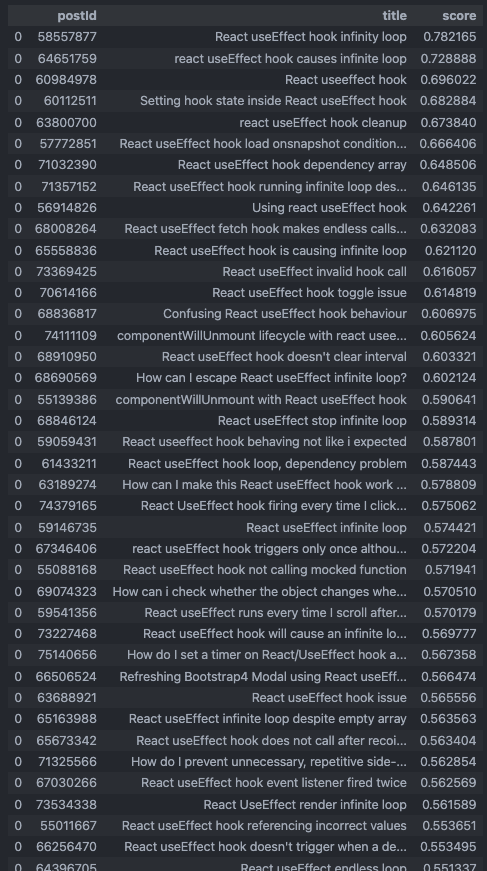
\includegraphics[scale=0.45]{assets/spacy-query-1-results.png}
  \noindent 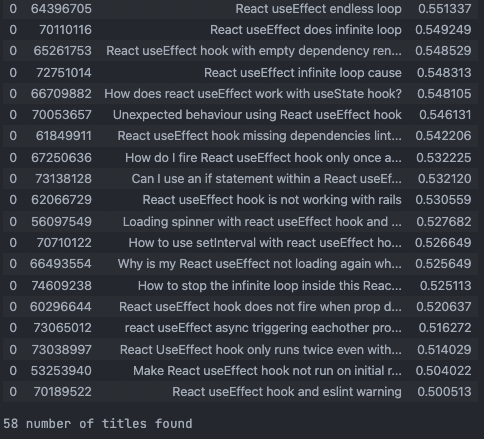
\includegraphics[scale=0.45]{assets/spacy-query-1-results-1.png}
\caption{Comparison of the results before and after removing stop words }\label{stopwords_comparison}
\end{figure}

\subsubsection{Remove Special Characters}
The next step is to remove special characters from the data. Since we're scrapping the data from StackOverflow directly with all sorts of special characters, the data is not clean at all. Having special characters in the dataset might causes a lot of unwanted trouble, therefore we decided to remove all special characters from the data. We've constructed a table \ref{table:special_character} to show all the special characters that we've found in the data. 

\begin{table}[ht]
  \caption{Special Character} % title of Table
  \centering % used for centering table
  \begin{tabular}{c c c c} % centered columns (4 columns)
  \hline\hline %inserts double horizontal lines
  Case & VoteCount & Dates & All Columns \\ [0.5ex] % inserts table
  %heading
  \hline % inserts single horizontal line
  1 & ( \, & , License: CC BY-SA 4.0 & segFault \\ % inserting body of the table
  2 & ) \, & ( \, &  \\
  3 & , & ) \ &  \\
  5 & ' & , & \\ [1ex] % [1ex] adds vertical space
  \hline %inserts single line
  \end{tabular}
  \label{table:special_character} % is used to refer this table in the text
\end{table}

We've used the string replace method to remove all special characters from the data.

Plot before and after here
\begin{figure}[H]
  \noindent 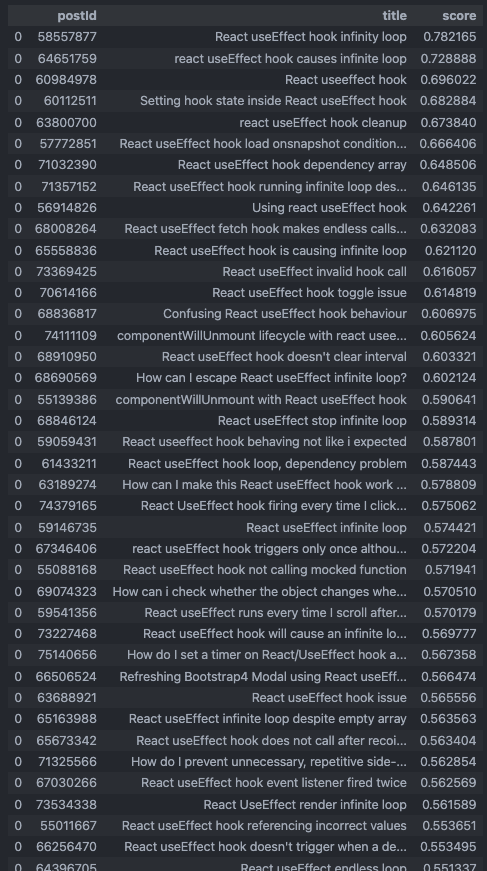
\includegraphics[scale=0.45]{assets/spacy-query-1-results.png}
  \noindent 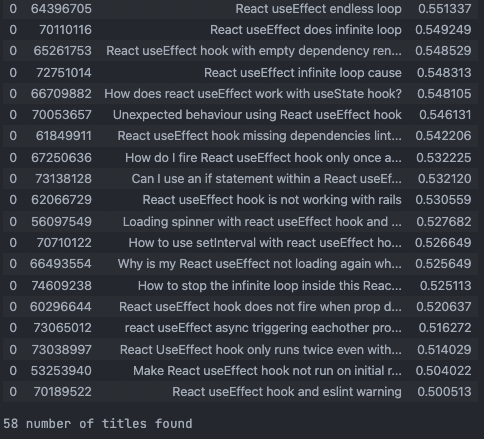
\includegraphics[scale=0.45]{assets/spacy-query-1-results-1.png}
\caption{Comparison of the results before and after removing stop words }\label{special_character_comparison}
\end{figure}

\subsubsection{Preprocessing - Extract URL from text}
It is essential to incorporate URLs into the data, as these may be mined for information on the context of the data. We are able to effortlessly extract the URLs from the data as it is scraped since the data contains HTML tags. The BeautifulSoup package was utilised so that we could access the URLs included inside the data. As a consequence of this, the url can be stored in a separate column of the dataset so that it can be referred to in the future.

In FYP 2, we are going to make an effort to put in place a system that can automatically determine the context relationships between retrieved URLs and extract more information from the URLs that have been obtained. Applying a score system is one way to determine whether or not the URL in question is relevant to the data. If the scoring method wasn't implemented, the process of the system going to each of the urls would take a very significant amount of time.

Plot before and after here
\begin{figure}[H]
  \noindent 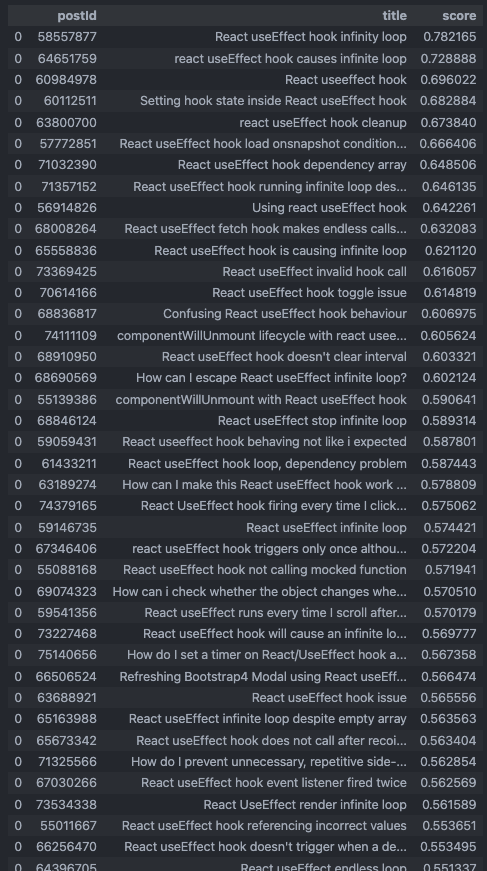
\includegraphics[scale=0.45]{assets/spacy-query-1-results.png}
  \noindent 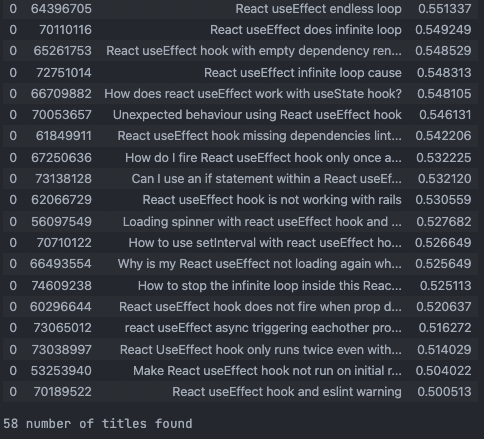
\includegraphics[scale=0.45]{assets/spacy-query-1-results-1.png}
\caption{Comparison of the results before and after extracting URLs }\label{url_extract_comparison}
\end{figure}

\subsubsection{Preprocessing - Remove Punctuation}
The next step is to remove punctuation from the data. Punctuation is usually surrounded by \texttt{``````} or \texttt{``````} in the data. We've used the string replace method to remove all punctuation from the data.

Plot before and after here
\begin{figure}[H]
  \noindent 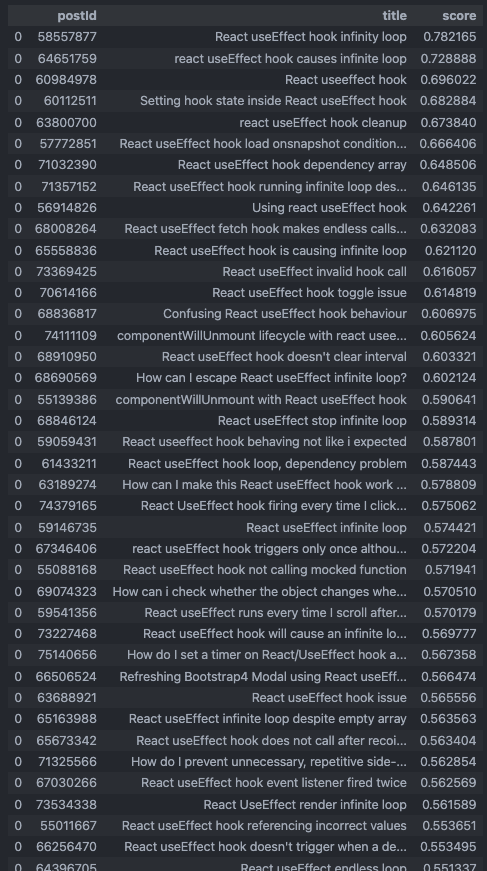
\includegraphics[scale=0.45]{assets/spacy-query-1-results.png}
  \noindent 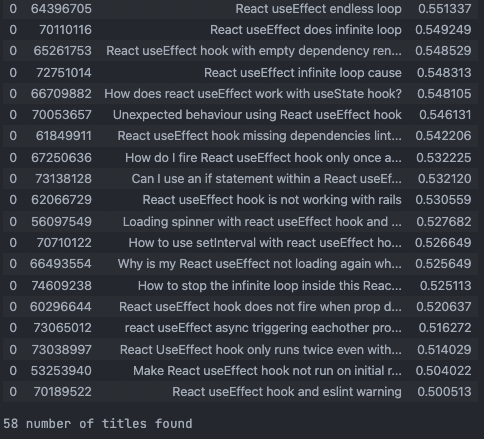
\includegraphics[scale=0.45]{assets/spacy-query-1-results-1.png}
\caption{Comparison of the results before and after removing punctuation }\label{punctuation_comparison}
\end{figure}

\subsubsection{Preprocessing - Remove code blocks}
The next step is to remove code blocks from the data. Code blocks are usually surrounded by \texttt{``````} or \texttt{``````} in the data. We've used the string replace method to remove all code blocks from the data.

Plot before and after here
\begin{figure}[H]
  \noindent 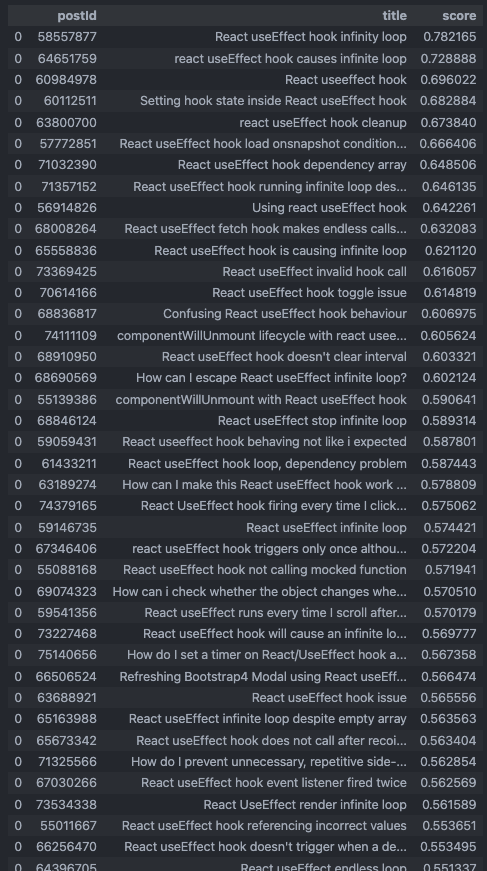
\includegraphics[scale=0.45]{assets/spacy-query-1-results.png}
  \noindent 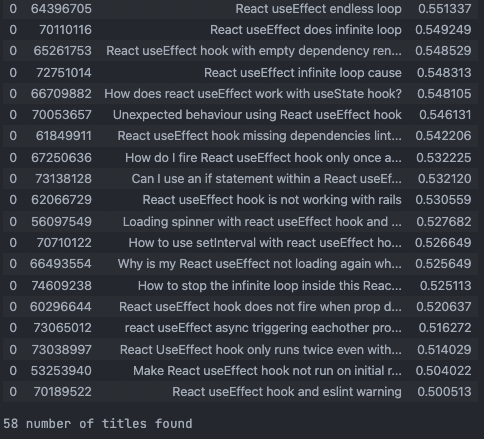
\includegraphics[scale=0.45]{assets/spacy-query-1-results-1.png}
\caption{Comparison of the results before and after removing code blocks }\label{code_block_comparison}
\end{figure}

\subsubsection{Preprocessing - Remove HTML Tags}
The next step is to remove HTML tags from the data. HTML tags are usually surrounded by \texttt{<} and \texttt{>} in the data. Again similarly to how we process code blocks, we've used the string replace method to remove all HTML tags from the data.

Plot before and after here
\begin{figure}[H]
  \noindent 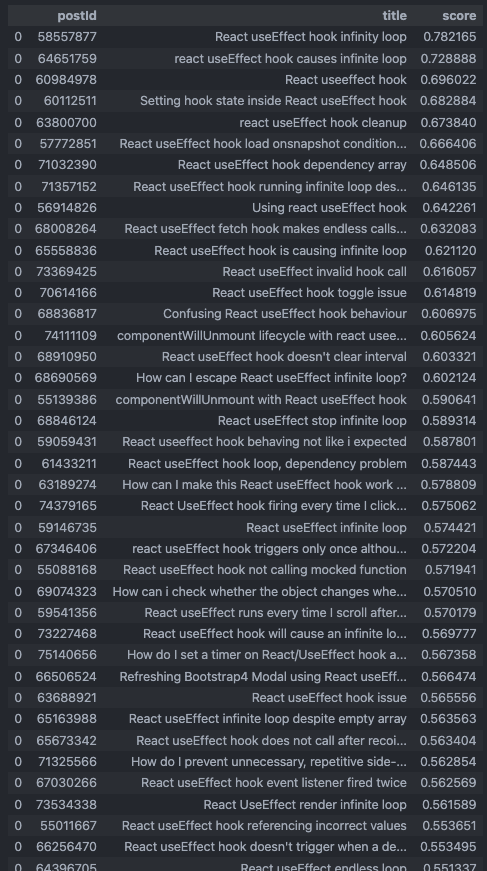
\includegraphics[scale=0.45]{assets/spacy-query-1-results.png}
  \noindent 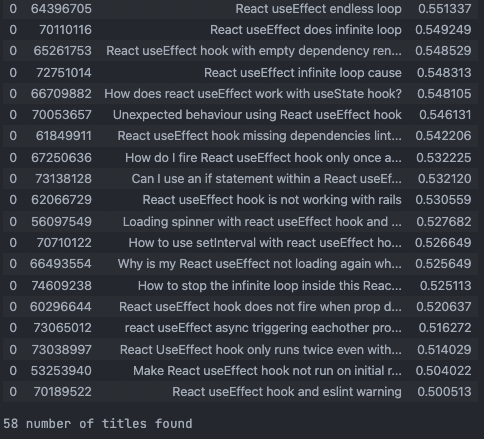
\includegraphics[scale=0.45]{assets/spacy-query-1-results-1.png}
\caption{Comparison of the results before and after removing HMTL Tags }\label{html_comparison}
\end{figure}

\subsubsection{Preprocessing - Stop Words Removal}
In the previous step \ref{sssec:preprocessing_finding_tech_related_stop_words},  we've found a list of stop words that are related to the technology domain. The removal is not done on the previous step because the text might contain noisy data Therefore, we decided to remove the stop words after the data is cleaned. We've used the string replace method to remove all stop words from the data.

Plot before and after here
\begin{figure}[H]
  \noindent 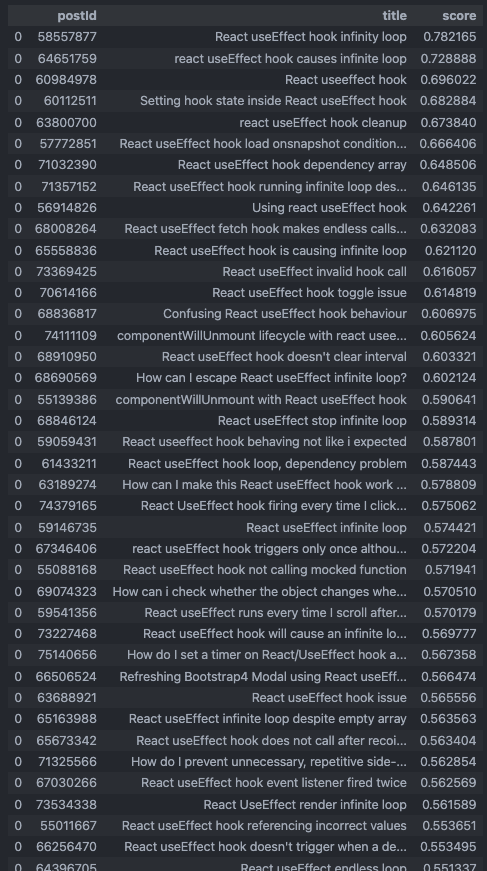
\includegraphics[scale=0.45]{assets/spacy-query-1-results.png}
  \noindent 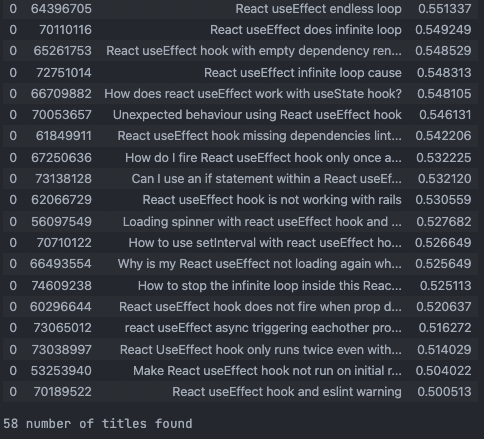
\includegraphics[scale=0.45]{assets/spacy-query-1-results-1.png}
\caption{Comparison of the results before and after removing stop words }\label{stop_words_comparison}
\end{figure}

\subsubsection{Preprocessing - Lemmatization/Stemming}
The process of truncating a word to it's root or base unit is called stemming or lemmatization. 

In the discipline of Natural Language Processing, text normalisation techniques like stemming and lemmatization are employed to get sentences, words, and documents ready for analysis. For instance, the terms "kick" and "kicked" are both forms of the verb "to kick," thus it's possible that you'll want your natural language processing application to recognise this. This is the idea of stripping down many uses of a term to its essential meaning.

Plot before and after here
\begin{figure}[H]
  \noindent 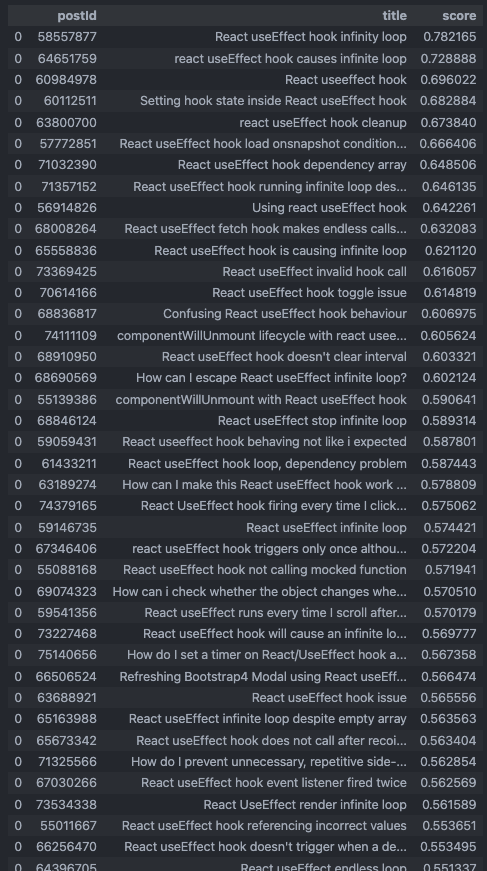
\includegraphics[scale=0.45]{assets/spacy-query-1-results.png}
  \noindent 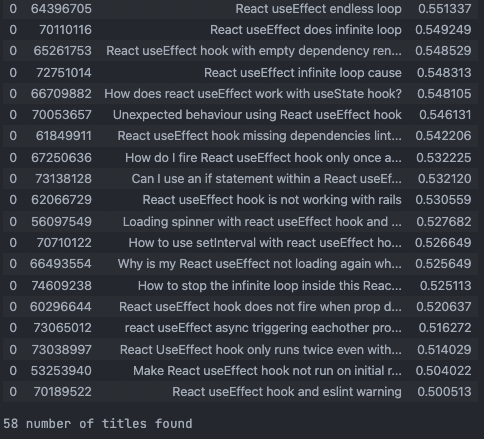
\includegraphics[scale=0.45]{assets/spacy-query-1-results-1.png}
\caption{Comparison of the results with using stemming or lemmatization }\label{stem_lem_comparison}
\end{figure}

\pagebreak
\noindent Techniques like lemmatization or stemming can be achieved by using the famous Python NLTK package.

However, whether to utilise stemming or lemmatization is a contentious issue. Because stemming is a primitive heuristic procedure that cuts off the ends of words in the aim of reaching this objective properly most of the time, it often involves the removal of derivational affixes. 

Lemmatization, on the other hand, is a more complex technique that takes into consideration morphological examination of the words. It does this by the use of a lexicon and morphological analysis of words, with the goal of removing only inflectional ends and returning the base or dictionary form of a word, known as the lemma.

To truly examine each of it's effectiveness on our dataset, we've made a comparison on which one is better. The result is shown below.

\noindent To conclude, we've decided to use lemmatization instead of stemming because we want to keep the words as much as possible for the summarization process.

\pagebreak
\subsubsection{Sentence Scoring}
At this stage, all of our sentences should be clean and ready to be scored. The scoring process is done by using the TF-IDF algorithm. The TF-IDF algorithm is a statistical measure that evaluates how relevant a word is to a document in a collection of documents. The algorithm is composed of two terms: the first computes the normalized Term Frequency (TF), aka. the number of times a word appears in a document, divided by the total number of words in that document; the second term is the Inverse Document Frequency (IDF), computed as the logarithm of the number of the documents in the corpus divided by the number of documents where the specific term appears.

The TF-IDF score is the product of these two terms. The TF-IDF score increases proportionally to the number of times a word appears in the document and is offset by the number of documents in the corpus that contain the word, which helps to adjust for the fact that some words appear more frequently in general.

The TF and IDF scores are defined as follows:

\begin{equation}
\label{eq:tf}
\text{TF} = \frac{\text{Number of times term t appears in a document}}{\text{Total number of terms in the document}}
\end{equation}

\begin{equation}
\label{eq:idf}
\text{IDF} = \log{\frac{\text{Total number of documents}}{\text{Number of documents with term t in it}}}
\end{equation}

At last, The TF-IDF scoring can be simplified into a single formula as shown below:

\begin{equation}
\label{eq:tfidf}
\text{TF-IDF} = \text{TF} \times \text{IDF}
\end{equation}

To apply the TF-IDF algorithm, we first join all the sentences into a single string. Then, we use the TF-IDF algorithm to calculate the TF-IDF score for each sentence and average it, thus the score will be tied with the post. The result is shown below.

\begin{figure}[H]
  \noindent 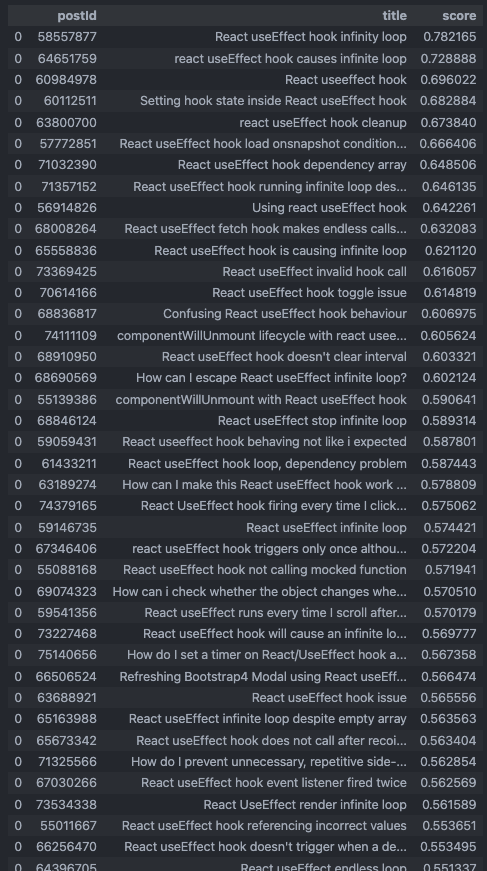
\includegraphics[scale=0.45]{assets/spacy-query-1-results.png}

\caption{Post scoring using sentence scoring }\label{scoring_sentence}
\end{figure}

\subsubsection*{Rank Post - 2nd Round}
After the sentence scoring process, we've got the score for each post. The next step is to rank the post based on the score. With that being said, an analysis and comparison can be done to compare the result of the first round and the second round. The result is shown below.

\begin{figure}[H]
  \noindent 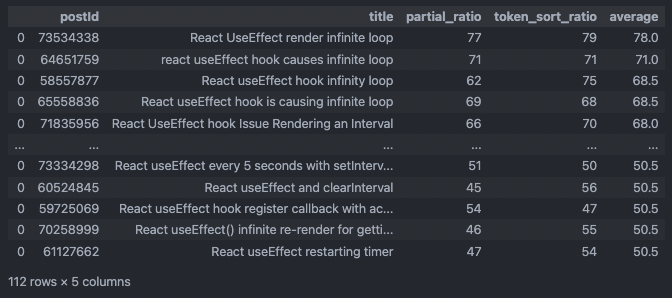
\includegraphics[scale=0.65]{assets/fuzzy-wuzzy-query-1-results.png}
\caption{Rank Post - 2nd Round}\label{rank_post_2nd_round}
\end{figure}

\pagebreak
\subsubsection{Sentiment Analysis}
Sentiment analysis is the process of determining whether a piece of writing is positive, negative, or neutral. It's also known as opinion mining, deriving the opinion or attitude of a speaker. A common use case of sentiment analysis is to discover how people feel about a particular topic.

Sentiment analysis is usually performed on textual data to help businesses monitor brand and product sentiment in customer feedback, and understand customer needs. It can also be used to gauge the sentiment of the general public to a particular event.

\textbf{But how does sentiment analysis take place in our framework? }

For context, each posts are scored based on the TF-IDF algorithm. The score is then used to rank the post. However the score itself is not telling enough to determine whether the post is useful or not. We've made an assumption that the post with a positive sentiment is more likely to be useful than the post with a negative sentiment. Therefore, we decided to use the sentiment analysis to determine the sentiment of the post. Therefore, we decided to use the sentiment analysis to add another layer of filtering ont he ranking aspect of the framework.

\subsubsection{Sentiment Analysis -- Model}
The model we've used is the famous twitter roberta base sentiment analysis model, which has been used over 2 million times this month. It is a RoBERTa base model trained on approximately 124M tweets from January 2018 to December 2021, and finetuned for sentiment analysis with the TweetEval benchmark. The model is able to predict and inference a probability score for each of the 3 classes: positive, negative, and neutral. 

Plot before and after here
\begin{figure}[H]
  \noindent 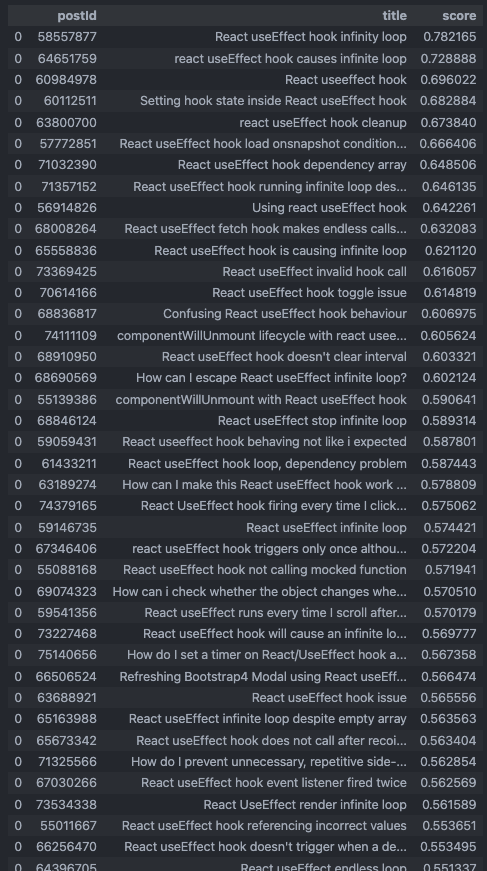
\includegraphics[scale=0.45]{assets/spacy-query-1-results.png}
\caption{Results using sentiment analysis }\label{sentiment_analysis_results}
\end{figure}

\pagebreak
\subsubsection{Rank Post}
After the sentiment analysis process, we've got the sentiment for each post. The next step is to rank the post based on the sentiment. This will be the third round of ranking. With the figures below, we can see the comparison between the first round, second round, and third round of ranking.

\begin{figure}[H]
  \noindent 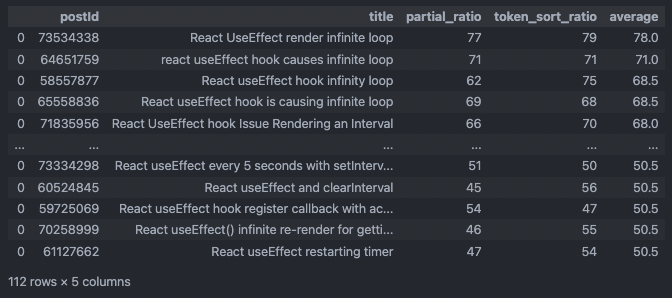
\includegraphics[scale=0.55]{assets/fuzzy-wuzzy-query-1-results.png}
  \noindent 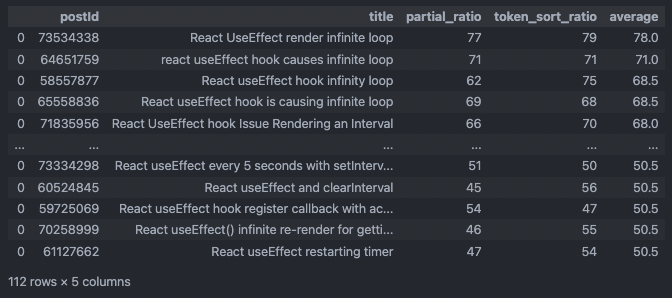
\includegraphics[scale=0.55]{assets/fuzzy-wuzzy-query-1-results.png}
  \noindent 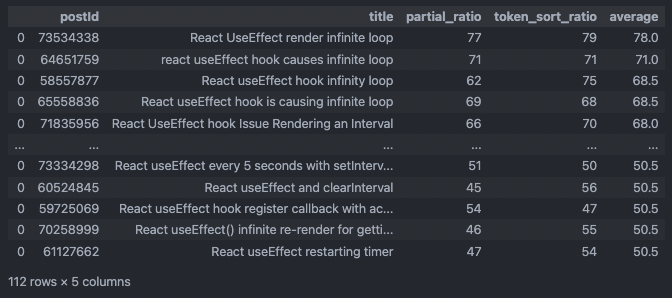
\includegraphics[scale=0.55]{assets/fuzzy-wuzzy-query-1-results.png}
\caption{Rank Post - 3rd Round}\label{rank_post_3rd_round}
\end{figure}


\subsubsection{Summarization}
At the final step, in order to fulfill a better user experience, the engine will then summarize the top 5 sentiment ranked posts. 

Summarization is the process of shortening a text document with software, in order to create a summary with the major points of the original document. As the name suggests, it is a technique to reduce the size of the given text while trying to retain the most important information. A summarization is crucial in our framework as it will help the user to understand the post better, faster and easier.
 
\subsubsection{Summarization -- Model} % quilbot
The model we've used is the very well known bart large cnn model, which has been used over 1 million times this month. BART model pre-trained on English language, and fine-tuned on CNN Daily Mail. It was introduced in the paper BART: Denoising Sequence-to-Sequence Pre-training for Natural Language Generation

BART is a transformer encoder-encoder (seq2seq) model with a bidirectional (BERT-like) encoder and an autoregressive (GPT-like) decoder. BART is pre-trained by (1) corrupting text with an arbitrary noising function, and (2) learning a model to reconstruct the original text.

BART is particularly effective when fine-tuned for text generation (e.g. summarization, translation) but also works well for comprehension tasks (e.g. text classification, question answering). This particular checkpoint has been fine-tuned on CNN Daily Mail, a large collection of text-summary pairs.

Plot before and after here
\begin{figure}[H]
  \noindent 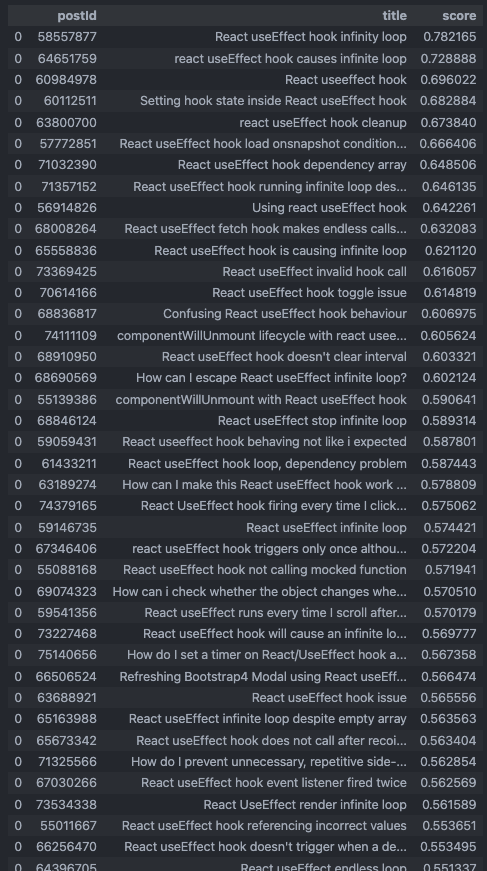
\includegraphics[scale=0.45]{assets/spacy-query-1-results.png}
\caption{Results after summarization }\label{summarization_results}
\end{figure}

\pagebreak
\subsubsection{The Finale: The Final Results}
We've come to the end of our framework using solution A. As you can see on the figure below, the result are promising, and the user is able to get the information they need with a very short text format. This helps the user to easily locate the posts that are useful to their query.

\begin{figure}[H]
  \noindent 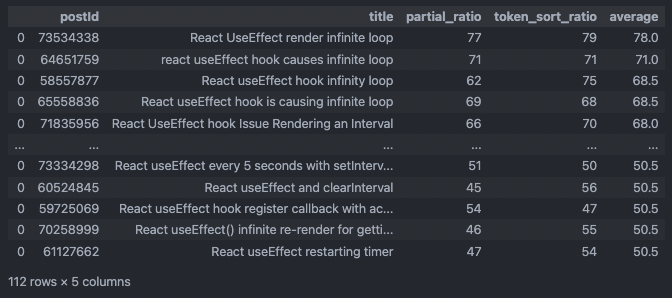
\includegraphics[scale=0.55]{assets/fuzzy-wuzzy-query-1-results.png}
\caption{Rank Post - The Finale }\label{finale_results_solution_a}
\end{figure}

\pagebreak
\subsection{Solution B}
The first solution focuses on ranking posts, whereby all comments, answers and answers comments are grouped together with the post and is been seen as a whole entity. Closed loop context, is the issue that we'll be addressing in this solution. We'll be explaining the architecture, the issue of solution A in detail, and the approach that we'll be taking to solve the issue.

\subsubsection{Solution B - Issue of Solution A}
The issue of solution A is the situation -- closed loop context, meaning that the ranking of the posts solely depends on the numbers, interactivity and the sentiment of the comments, answers and answers comments of the post. 

This is not a serious problem, however there is room for improvement. Jumping on another point of view, let's zoom out from the post context, let's view all of the comments, answers, and answer comments all together from every posts. The argument that we're trying to define here is, there is possibility that the answers from other posts are more relevant to the query than the answers from the post itself? The sole reason where the post that contains the better answers is not ranked is because the title of the post is not relevant to the query.

This is where the second solution comes in. We'll be using the same approach as solution A, however we'll be grouping all related answers across all posts and do string similarity, and the rest of the architecture will be more or less similar to solution A. 

Note, this is a solution made up with an assumption of the possibility of the answers from other posts are more relevant to the query than the answers from the post itself. The actual implementation will be covered in FYP2. 

\subsubsection{Solution B - Architecture}
The architecture of solution B is very similar to solution A, the only difference is that we'll be grouping all related answers across all posts, we can see that in the figure \ref*{solution_b_architecture}

\pagebreak
\begin{figure}[H]
  \centering
  \noindent 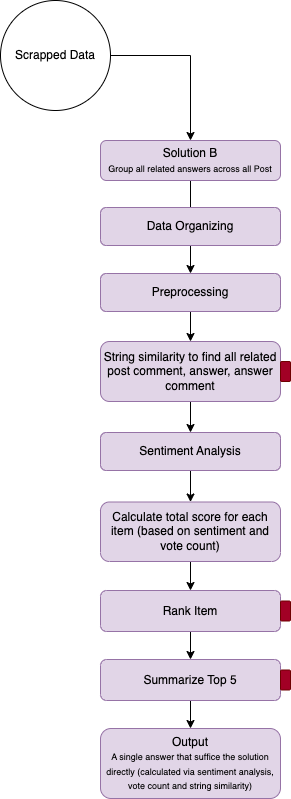
\includegraphics[scale=0.85]{assets/solution-b.png}
\caption{Solution B Architecture }\label{solution_b_architecture}
\end{figure}

\subsubsection{Solution B - Approach}
The approach that we'll be taking is very similar to solution A, the only differentiating factor is that we're thinking on a wider context, we're not just thinking about the post itself, we're thinking about all the posts. All of the comments should be seen as equal no matter the parent post of the comments itself. 

Data cleaning \ref{data-cleaning}, organizing \ref*{data-organization}, pre-processing \ref*{sssec:preprocessing_finding_tech_related_stop_words} will be done in the same way as solution A.  Just that the data will not be grouped by post \ref*{grouped_by_post}, but rather by all posts. 

This way all comments, answers, answers comments take a part in the ranking process. We believe that this is a better system as it excludes the bias of the post title, and it helps to rank the individual item that are more relevant to the query, eventually leading to a better user experience.

\section{Topic Modeling}


\section{Real Time Capabilities Issue} \label{real-time-capabilities}
One of the big issues for this framework to be generalized is the dataset. The dataset has to be generalized enough to be able to answer any query, that is simply impossible considering the wide range of the tehcnical field.

Real time scraping to populate the dataset is not a good idea as it will be very costly, time consuming, and cpu intensive, as our workers have to scale up to the demand of the users. 

Therefore, we've came up with two solutions to solve the problem, the first solution is to build a FAQs repository to store FAQs for further usage, and the second solution is to predict the next faq that will be asked.

\pagebreak
\section{FAQs Repository}~\label{faq-repo}
With the first solution, a FAQs repository is needed to be built. The FAQs repository will be a collection of questions and answers that are related to the technical field. The way it works is that whenever a user asks a question, the system will check if the question is in the FAQs repository, if it is, the system will return the answer from the FAQs repository. If it's not, the system will then scrap all the related posts from stackoverflow, and do inferencing. The summarized result will be stored in the FAQs repository, and the user or anyone will be able to access the answer from the FAQs repository next time they ask the same question.

\section{FAQs Repository - Architecture} 
In the below figure, we can see the architecture of the FAQs repository. The FAQs repository is a database that stores the questions and answers. The database is populated by the system, and the system will check the database whenever a user asks a question.

\pagebreak
\begin{figure}[H]
  \centering
  \noindent 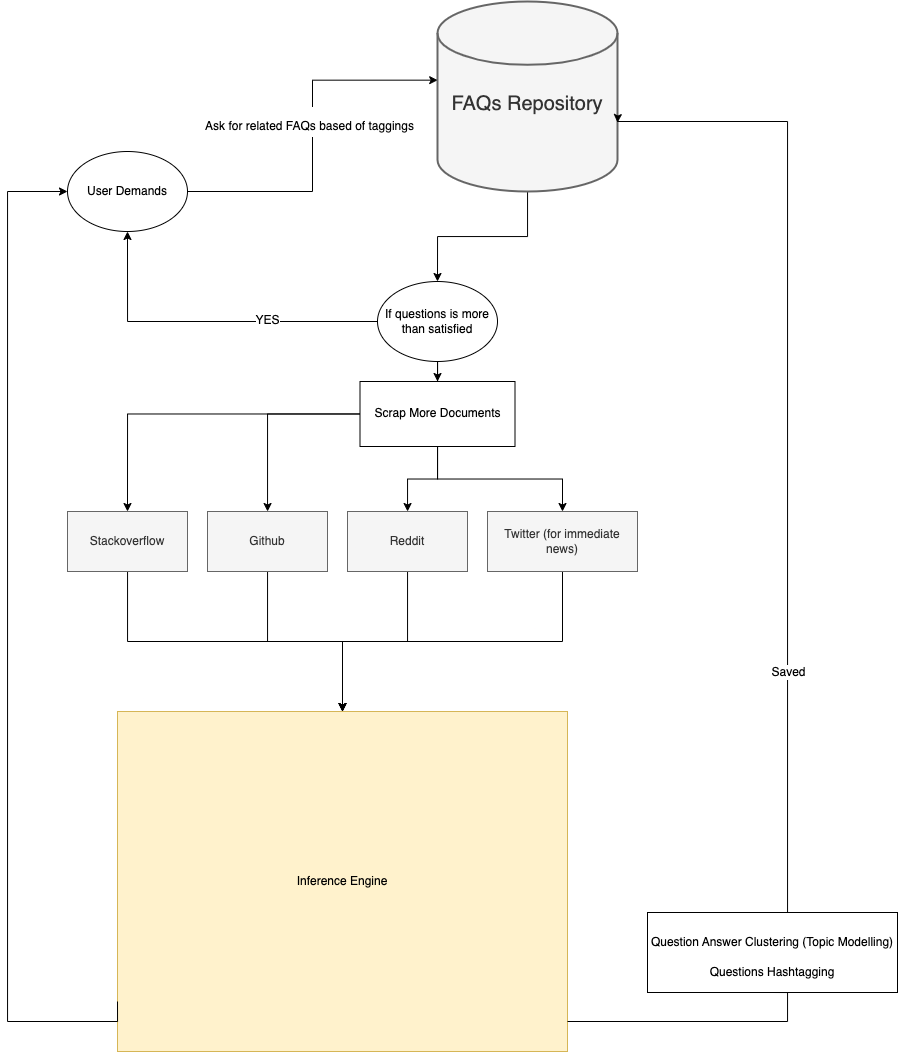
\includegraphics[scale=0.50]{assets/faq_repo_workflow.png}
\caption{FAQ Repository Architecture}\label{faq_repo_architecture}
\end{figure}

\section{FAQs Repository - Approach}
With the above architecture, the system will be functioning as stated below:

1. The user asks a question

2. The system will check if the question is in the FAQs repository

3. If the question is in the FAQs repository, the system will return the answer from the FAQs repository

4. If the question is not in the FAQs repository, the system will then scrap all the related posts from stackoverflow, and do inferencing

5. The summarized result will be stored in the FAQs repository, and the user or anyone will be able to access the answer from the FAQs repository next time they ask the same question.

With this architecture, we can ensure that the system is not only able to answer the question that is asked before, but also able to answer the question that is not asked before, also it can ensure that the system will not scrap the same question again and again, as it's already in the FAQs repository.

\section{FAQs Repository - Database Design}
The database of choice is MongoDB, as it's a NoSQL database, and it's very easy to scale up. As a plus point, MongoDB being a NoSQL database gives us the flexibility to store the data in anyway we wanted, and the structure of the data can be altered whenever. 

The database will be structured as below:
\pagebreak
\begin{figure}[H]
  \centering
  \noindent 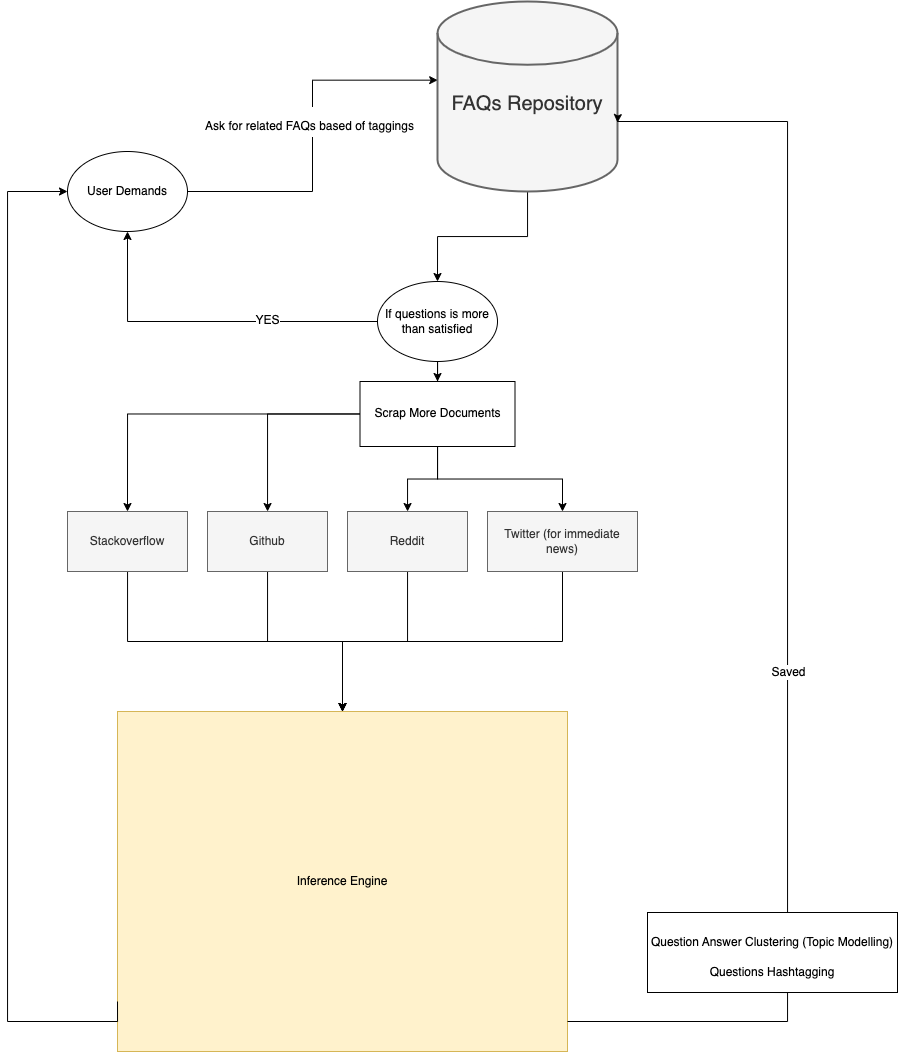
\includegraphics[scale=0.50]{assets/faq_repo_workflow.png}
\caption{Database Design}\label{database_design}
\end{figure}

\section{FAQs Repository - System Design}
An system design figure is shown below:

\pagebreak
\begin{figure}[H]
  \centering
  \noindent 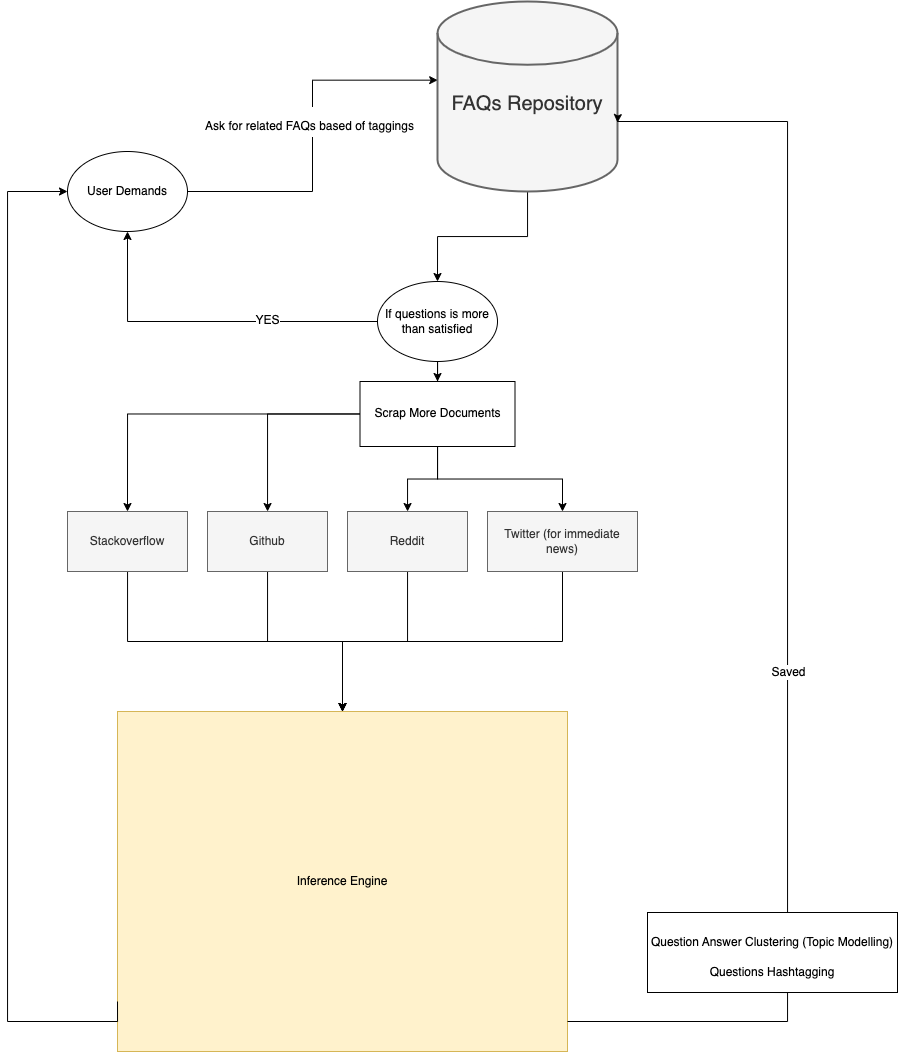
\includegraphics[scale=0.50]{assets/faq_repo_workflow.png}
\caption{System Design}\label{system_design}
\end{figure}

The entire backend will be built using NodeJs, as it's a very popular language, and it's very easy to scale. We'll be using a boilerplate created by the author of this thesis, which consists of multi-threading and clustering capabilities. These factors will help us to scale up the system whenever we need to. The boilerplate is available at \url{https://github.com/Shaunmak1214/cluster-node-auth-sql-boilerplate.git}. 

A few notable perks that the boilerplate has is that it has a built in authentication system, and it has a built in SQL database, and a whole lot more. All of the important features of the boilerplate will be listed below:

\begin{itemize}
  \item {Clustering in Node.js}
  \item {Server with Express.js}
  \item {Database schema and models using Sequelize ORM}
  \item {User authentication with JWT}
  \item {StandardJs for coding standards and styling}
  \item {Request validation using Express-validator}
  \item {Morgan and Winston for server side logging}
  \item {Swagger for API documentation}
\end{itemize}

To host the backend, we'll be using AWS EC2, as it's the best cheap option, and it's very easy to scale according to user demands. Amazon Elastic Compute Cloud (Amazon EC2) offers the broadest and deepest compute platform, with over 500 instances and choice of the latest processor, storage, networking, operating system, and purchase model to help you best match the needs of your workload. We are the first major cloud provider that supports Intel, AMD, and Arm processors, the only cloud with on-demand EC2 Mac instances, and the only cloud with 400 Gbps Ethernet networking. We offer the best price performance for machine learning training, as well as the lowest cost per inference instances in the cloud. More SAP, high performance computing (HPC), ML, and Windows workloads run on AWS than any other cloud.

Laslty to protect the servers from ddos attacks, we'll be using AWS WAF, which is a web application firewall that helps protect your web applications from common web exploits that could affect application availability, compromise security, or consume excessive resources. AWS WAF gives you control over which traffic to allow or block to your web applications by defining customizable web security rules. You can use AWS WAF to create security rules that block common attack patterns, such as SQL injection or cross-site scripting, and rules that filter specific types of traffic. AWS WAF is integrated with AWS Shield, a managed DDoS protection service that safeguards web applications running on AWS. AWS Shield Standard provides always-on detection and automatic inline mitigations that minimize application downtime and latency, and AWS Shield Advanced provides distributed denial of service (DDoS) attack protection, proactive engagement with AWS support, and usage metrics.

\section{CronJobs - Predictive FAQ Generation System}
While the first solution -- FAQ Repository \ref*{faq-repo} is able to solve the problem, there's still one big problem. The FAQs repository solution works well if your question is already asked by someone, but what if your question is not asked by anyone before? The system will not be able to answer your question, and you will have to wait for the lenghty process for the system to scrap, process, analyze, rank and summarize the data for you. This is not ideal, if you have tons of bugs to solve and you have to wait for the system to answer your question.

To solve this problem, we'll be using a cronjob to run the system every 24 hours, and the system will scrap, process, analyze, rank and summarize the data, and store it in the FAQs repository. This way, the system will be able to answer any question that is asked by the user, and the user will not have to wait for the system to answer their question.

One of the big question mark for this is, what to scrap? 

For context, we have primarily 4 data sources, Stackoverflow, Reddit, Twitter and lastly Github. 

\section{CronJobs - Predictive FAQ Generation System - Architecture}
\newpage
\begin{landscape}
\begin{figure}[t]
  \noindent 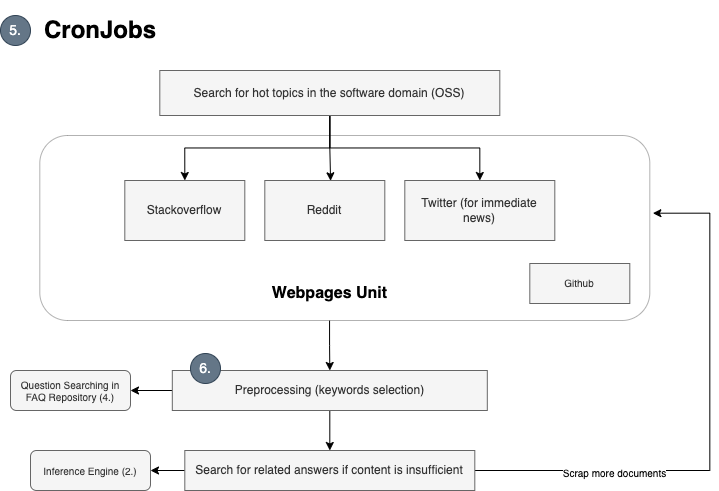
\includegraphics[scale=0.4, angle=0]{assets/cron_job_workflow.png}
\caption{CronJobs Architecture}\label{cronjobs_architecture}
\end{figure}
\end{landscape}
\newpage

\section{CronJobs - Predictive FAQ Generation System - Approach}
With the above architecture, the system will be functioning as stated below:

1. The system will scrap all the posts from stackoverflow, reddit, twitter and github every 24 hours

2. Perform topic modeling on the scrapped data, Extracting keywords

3. If dataset is not sufficient (metrics will be explored), scrap more documents related to the topic. 

4. Process, analyze, rank and summarize the data 

5. Store the summarized data in the FAQs repository

Which the proposed architecture, we can improve the system where the system will populate itself with the most recent data, and in the hopes where the system is able to fit with the user's needs.

\section{Result Analysis} 

\section{Evaluation} 

\section{Future Work} 